% Compile with PdfLaTeX

\documentclass[12pt,letterpaper,boxed]{hmcpset}

% set 1-inch margins in the document
\usepackage[margin=1in]{geometry}

% include this if you want to import graphics files with /includegraphics
\usepackage{enumerate}
\usepackage{graphicx}
\usepackage{amsmath,amssymb}
\usepackage[all]{xy}

\usepackage[usenames,dvipsnames]{color}
\usepackage[colorlinks,linkcolor=NavyBlue,anchorcolor=red,citecolor=green]{hyperref}
\usepackage{mathrsfs}
\usepackage{cancel}
\usepackage{cite}
\usepackage{setspace}
\usepackage{tikz}


\usepackage{mathtools}
\DeclarePairedDelimiter\ceil{\lceil}{\rceil}
\DeclarePairedDelimiter\floor{\lfloor}{\rfloor}



\renewcommand{\baselinestretch}{1.05} 

\renewcommand\appendix{\setcounter{secnumdepth}{-2}}

\newcommand{\Obj}{\mathrm{Obj}} 
\newcommand{\Hom}{\mathrm{Hom}} 
\newcommand{\GL}{\mathrm{GL}} 
\newcommand{\SL}{\mathrm{SL}} 
\newcommand{\Aut}{\mathrm{Aut}}
\newcommand{\Inn}{\mathrm{Inn}}
\newcommand{\Grp}{\mathsf{Grp}} 
\newcommand{\Set}{\mathsf{Set}}
\newcommand{\Ab}{\mathsf{Ab}}  
\newcommand{\R}{\mathbb{R}} 
\newcommand{\C}{\mathbb{C}}
\newcommand{\Q}{\mathbb{Q}}
\newcommand{\Z}{\mathbb{Z}}
\newcommand{\N}{\mathbb{N}}


% info for header block in upper right hand corner
\name{Huyi Chen}
\updatedate{\today}

\begin{document}
		
\problemlist{\textbf{Algebra, Chapter 0}\\By Paolo Aluffi}

\tableofcontents
\appendix

\section{Chapter I.\quad Preliminaries: Set theory and categories}

\subsection{\textsection1. Naive Set Theory}

\begin{problem}[1.6]
Define a relation $\sim$ on the set $\mathbb{R}$ of real numbers, by setting $a\sim b\iff b-a \in\mathbb{Z}$. Prove that this is an equivalence relation, and find a \textquoteleft compelling' description for $\mathbb{R}/\sim$. Do the same for the relation $\approx$ on the plane $\mathbb{R}\times\mathbb{R}$ defined by declaring $(a_1, a_2)\approx(b_1, b_2)\iff b_1-a_1 \in\mathbb{Z}$ and $b_2-a_2 \in\mathbb{Z}$. [\textsection II.8.1, II.8.10]
\end{problem}
\begin{solution}
Imaginatively, $\mathbb{R}/\sim$ can be viewed as a ring of length 1 by bending the real line $\mathbb{R}$.	Then we can rotate a ring around an axis of rotation to get $\mathbb{R}\times\mathbb{R}/\approx$, which makes a torus.
\end{solution}	




\subsection{\textsection2. Functions between sets}

\begin{problem}[2.1]
How many different bijections are there between a set $S$ with $n$ elements
and itself? [\textsection II.2.1]
\end{problem}
\begin{solution}
	There are $n!$ different bijections $S\rightarrow S$.
\end{solution}


\subsection{\textsection3. Categories}
\begin{problem}[3.1]
	Let $\mathsf{C}$ be a category. Consider a structure $\mathsf{C}^{op}$ with:
	\begin{itemize}
	\item $\Obj(\mathsf{C}^{op}) := \Obj(\mathsf{C})$;
	\item for $A$, $B$ objects of $\mathsf{C}^{op}$ (hence, objects of $\mathsf{C}$), $\Hom_{\mathsf{C}^{op}} (A,B) := \Hom_\mathsf{C}(B,A)$
	\end{itemize}
	Show how to make this into a category (that is, define composition of morphisms
	in $\mathsf{C}^{op}$ and verify the properties listed in \textsection3.1).
	Intuitively, the 'opposite' category $\mathsf{C}^{op}$ is simply obtained by 'reversing all the
	arrows' in C. [5.1, \textsection VIII.1.1, \textsection IX.1.2, IX.1.10]
\end{problem}
\begin{solution}
	\begin{itemize}
		\item For every object $A$ of $\mathsf{C}$, there exists one identity morphism $1_A\in\Hom_\mathsf{C}(A,A)$. Since $\Obj(\mathsf{C}^{op}) := \Obj(\mathsf{C})$ and $\Hom_{\mathsf{C}^{op}} (A,A) := \Hom_\mathsf{C}(A,A)$, for every object $A$ of $\mathsf{C}^{op}$, the identity on $A$ coincides with $1_A\in\mathsf{C}$. 
		\item For $A$, $B$, $C$ objects of $\mathsf{C}^{op}$ and $f\in\Hom_{\mathsf{C}^{op}} (A,B)=\Hom_\mathsf{C}(B,A)$, $g\in\Hom_{\mathsf{C}^{op}} (B,C)=\Hom_\mathsf{C}(C,B)$, the composition laws in $\mathsf{C}$ determines a morphism $f*g$ in $\Hom_{\mathsf{C}} (C,A)$, which deduces the composition defined on $\mathsf{C}^{op}$:
		\[
		\begin{aligned}
		\Hom_{\mathsf{C}^{op}} (A,B)\times\Hom_{\mathsf{C}^{op}} (B,C)&\longrightarrow \Hom_{\mathsf{C}^{op}} (A,C)\\
		(f,g)&\longmapsto g\circ f:=f*g
		\end{aligned}
		\]
		\item Associativity. If $f\in\Hom_{\mathsf{C}^{op}} (A,B)$, $g\in\Hom_{\mathsf{C}^{op}} (B,C)$, $h\in\Hom_{\mathsf{C}^{op}} (C,D)$, then
		\[
		f\circ(g\circ h)=f\circ(h*g)=(h*g)*f=h*(g*f)=(g*f)\circ h=(f\circ g)\circ h.
		\]
		\item Identity. For all $f\in\Hom_{\mathsf{C}^{op}} (A,B)$, we have
		\[
		f\circ 1_A=1_A*f=f,\quad 1_B\circ f=f*1_B=f.
		\]
	\end{itemize}
	Thus we get the full construction of $\mathsf{C}^{op}$.
\end{solution}

\begin{problem}[3.3]
	$\vartriangleright$ Formulate precisely what it means to say that $1_a$ is an identity with respect to composition in Example 3.3, and prove this assertion. [\textsection3.2]
\end{problem}
\begin{solution}
	Suppose $S$ is a set, and $\sim$ is a relation on $S$ satisfying the reflexive and transitive property. Then we can encode this data into a category $\mathsf{C}$:
	\begin{itemize}
		\item Objects: the elements of $S$;
		\item Morphisms: if $a, b$ are objects (that is: if $a, b \in S$) then let $\Hom(a, b)$ be the set consisting of the element $(a, b) \in S \times S$ if $a \sim b$, and $\Hom(a, b) = \varnothing$.
		otherwise.
	\end{itemize}
    Given the composition of two morphisms
	\begin{align*}
		\Hom_\mathsf{C}(A,B) \times\Hom_\mathsf{C}(B,C)&\longrightarrow\Hom_\mathsf{C}(A,C)\\
		(a,b)\circ(b,c)&\longmapsto(a,c)
	\end{align*}
	we are asked to check $1_a = (a, a)$ is an identity with respect
	to this composition.
\end{solution}
\subsection{\textsection4. Morphisms}
\begin{problem}[4.2]
	In Example 3.3 we have seen how to construct a category from a set endowed	with a relation, provided this latter is reflexive and transitive. For what types of relations is the corresponding category a groupoid (cf. Example 4.6)? [\textsection4.1]
\end{problem}
\begin{solution}
    For a reflexive and transitive relation $\sim$ on a set $S$, define the category $\mathsf{C}$ as follows:
    \begin{itemize}
    	\item Objects: $\mathrm{Obj}(\mathsf{C})=S$;
    	\item Morphisms: if $a, b$ are objects (that is: if $a, b \in S$) then let 
    	\[
    	\mathrm{Hom}_\mathsf{C}(a, b)=
    	\left\{
    	\begin{aligned}
    	&(a, b)\in S\times S &\text{ if } a\sim b\\	
    	& \varnothing &\text{ otherwise}\\
    	\end{aligned}
    	\right.
    	\]
    \end{itemize}
    In Example 3.3 we have shown the category. If the relation $\sim$ is endowed with symmetry, we have
    \[
    (a,b)\in\mathrm{Hom}_\mathsf{C}(a, b)\implies a\sim b\implies b\sim a\implies (b,a)\in\mathrm{Hom}_\mathsf{C}(b, a).
    \]
    Since
    \[
    (a,b)(b, a)=(a,a)=1_a,\quad(b, a)(a,b)=(b,b)=1_b,
    \]
    in fact $(a,b)$ is an isomorphism. From the arbitrariness of the choice of $(a,b)$, we show that $\mathsf{C}$ is a groupoid. Conversely, if $\mathsf{C}$ is a groupoid, we can show the relation $\sim$ is symmetric. To sum up, the category $\mathsf{C}$ is a groupoid
    if and only if the corresponding relation $\sim$ is an equivalence relation.
\end{solution}

\subsection{\textsection5. Universal properties}
\begin{problem}[5.1]
	Prove that a final object in a category $\mathsf{C}$ is initial in the opposite category $\mathsf{C}_{op}$	(cf. Exercise 3.1).
\end{problem}
\begin{solution}
	An object $F$ of $\mathsf{C}$ is final in $\mathsf{C}$ if and only if
	\[
	\forall A \in \Obj(\mathsf{C}) : \Hom_\mathsf{C}(A,F) \text{ is a singleton.}
	\]
	That is equivalent to
	\[
	\forall A \in \Obj(\mathsf{C}_{op}) : \Hom_{\mathsf{C}_{op}}(F,A) \text{ is a singleton,}
	\]
	which means $F$ is initial in the opposite category $\mathsf{C}_{op}$.	
\end{solution}

\section{Chapter II.\quad Groups, first encounter}

\subsection{\textsection1. Definition of group}
\begin{problem}[1.1]
	Write a careful proof that every group is the group of isomorphisms of a groupoid. In particular, every group is the group of automorphisms of some object in some category.
\end{problem}
\begin{solution}
	Assume $G$ is a group. Define a category $\mathsf{C}$ as follows:
	\begin{itemize}
		\item Objects: $\mathrm{Obj}(\mathsf{C})=\{*\}$;
		\item Morphisms: $\mathrm{Hom}_\mathsf{C}(*,*)=\mathrm{End}_\mathsf{C}(*)=G$.
	\end{itemize}	
	The composition of homomorphism is corresponding to the multiplication between two elements in $G$. The identity morphism on $*$ is $1_*=e_G$, which satisfies for all $g\in \mathrm{Hom}_\mathsf{C}(*,*)$,
	\[
	ge_G=e_Gg=g,
	\]
	and
	\[
	gg^{-1}=e_G,\;g^{-1}g=e_G.
	\]
	Thus any homomorphism $g\in \mathrm{Hom}_\mathsf{C}(*,*)$ is an isomorphism and accordingly $\mathsf{C}$ is a groupoid. Now we see $G=\mathrm{End}_\mathsf{C}(*)$ is the group of isomorphisms of a groupoid. Moreover, supposing that $*$ is an object in some category $\mathsf{D}$, $G$ would be the group of automorphisms of $*$, which is denoted as $\mathrm{Aut}_\mathsf{D}(*)$.
\end{solution}

\begin{problem}[1.4]
	Suppose that $g^2 = e$ for all elements $g$ of a group $G$; prove that $G$ is commutative.
\end{problem}
\begin{solution}
	For all $a,b\in G$,
	\[
	abab=e\implies a(abab)b=ab\implies (aa)ba(bb)=ab\implies ba=ab.
	\]
\end{solution}

\subsection{\textsection2. Examples of groups}
\begin{problem}[2.1]
	One can associate an $n\times n$ matrix $M_\sigma$ with a permutation $\sigma \in S_n$, by
	letting the entry at $(i, \sigma(i))$ be 1, and letting all other entries be 0. For example,
	the matrix corresponding to the permutation
	\[
	\sigma=\left(
	\begin{matrix}	
	1 & 2 & 3\\	
    3 & 1 & 2	
	\end{matrix}
	\right)\in S_3
	\]
	would be 
	\[
	M_\sigma=\left(
	\begin{matrix}	
	0 & 0 & 1\\	
	1 & 0 & 0\\	
	0 & 1 & 0
	\end{matrix}
	\right)
	\]
	Prove that, with this notation,
	\[
	M_{\sigma\tau}=M_{\sigma}M_{\tau}
	\]
	for all $\sigma,\tau\in S_n$, where the product on the right is the ordinary product of matrices.
\end{problem}
\begin{solution}
	By introducing the Kronecker delta function	
    \[
    \delta _{{i,j}}=
    	\begin{cases}
    	0{\text{\quad if }}i\neq j,\\
    	1{\text{\quad if }}i=j,
    	\end{cases}
    \]
	the entry at $(i,j)$ of the matrix $M_{\sigma\tau}$ can be written as
	\[
	(M_{\sigma\tau})_{i,j}=\delta_{\tau(\sigma(i)),j}
	\]
	and the entry at $(i,j)$ of the matrix $M_{\sigma}M_{\tau}$ can be written as
	\[
	(M_{\sigma}M_{\tau})_{i,j}=\sum_{k=1}^{n}(M_{\sigma})_{i,k}(M_{\tau})_{k,j}=\sum_{k=1}^{n}\delta_{\sigma(i),k}\cdot\delta_{\tau(k),j}=\sum_{k=1}^{n}\delta_{\sigma(i),k}\cdot\delta_{k,\tau^{-1}(j)}=\delta_{\sigma(i),\tau^{-1}(j)},
	\]
	where the last but one equality holds by the fact 
	\[
	\tau(k)=j\iff k=\tau^{-1}(j).
	\]
	Noticing that
	\[
	\tau(\sigma(i))=j\iff \sigma(i)=\tau^{-1}(j),
	\]
    we see $M_{\sigma\tau}=M_{\sigma}M_{\tau}$
    for all $\sigma,\tau\in S_n$.
\end{solution}


\begin{problem}[2.2]
	Prove that if $d \le n$, then $S_n$ contains elements of order $d$.
\end{problem}
\begin{solution}
	The cyclic permutation 
	\[
	\sigma=(1\;2\;3\cdots d)
	\]
    is an element of order $d$ in $S_n$.
\end{solution}



\begin{problem}[2.3]
	For every positive integer $n$ find an element of order $n$ in $S_\mathbb{N}$.
\end{problem}
\begin{solution}
The cyclic permutation 
\[
\sigma=(1\;2\;3\cdots n)
\]
is an element of order $d$ in $S_n$.
\end{solution}



\begin{problem}[2.4]	
	Define a homomorphism $D_8 \rightarrow S_4$ by labeling vertices of a square, as we did
	for a triangle in \textsection2.2. List the 8 permutations in the image of this homomorphism.
\end{problem}
\begin{solution}
	The image of $n$ rotations under the homomorphism are
	\[
	\sigma_1=e_{D_8},\;\sigma_2=(1\;2\;3\;4),\;\sigma_3=(1\;3)(2\;4),\;\sigma_4=(1\;4\;3\;2).
	\]
	The image of $n$ reflections under the homomorphism are
	\[
	\sigma_5=(1\;3),\;\sigma_6=(2\;4),\;\sigma_7=(1\;2)(3\;4),\;\sigma_8=(1\;4)(3\;2).
	\]
\end{solution}



\begin{problem}[2.11]	
	Prove that the square of every odd integer is congruent to 1 modulo 8.
\end{problem}
\begin{solution}
	Given an odd integer $2k+1$, we have
	\[
	(2k+1)^2=4k(k+1)+1,
	\]
	where $k(k+1)$ is an even integer. So $(2k+1)^2\equiv1\mod 8$.
\end{solution}



\begin{problem}[2.12]	
	Prove that there are no integers $a, b, c$ such that $a^2+b^2=3c^2$. (Hint: studying the equation $[a]^2_4+[b]^2_4=3[c]^2_4$ in $\mathbb{Z}/4\mathbb{Z}$, show that $a, b, c$ would all have to be even. Letting $a=2k, b=2l,c=2m$, you would have $k^2+l^2=3m^2$. What's wrong with that?)
\end{problem}
\begin{solution}
	\[
	a^2+b^2=3c^2\implies [a]^2_4+[b]^2_4=3[c]_4^2.
	\]
	Noting that $[0]^2_4=[0]_4,[1]^2_4=[1]_4,[2]^2_4=[0]_4,[3]^2_4=[1]_4$, we see $[c]_4^2$ must be $[0]_4$ and so do $[a]_4^2$ and $[b]_4^2$. Hence  $[a]_4,[b]_4,[b]_4$ can only be $[0]_4$ or $[2]_4$, which justifies letting $a=2k_1, b=2l_2,c=2m_1$. After substitution we have $k^2+l^2=3m^2$. Repeating this process $n$ times yields $a=2^nk_n, b=2^nl_n,c=2^nm_n$. For a sufficiently large number $N$, the absolute value of $k_N,l_N,m_N$ must be less than 1. Thus we conclude that $a=b=c=0$ is the unique solution to the equation $a^2+b^2=3c^2$.
\end{solution}
    


\begin{problem}[2.13]	
	Prove that if $\gcd(m, n) = 1$, then there exist integers $a$ and $b$ such that $am + bn = 1$. (Use Corollary 2.5.) Conversely, prove that if $am+ bn = 1$ for some integers $a$ and $b$, then $\gcd(m, n) = 1$. [2.15, \textsection V.2.1, V.2.4]
\end{problem}
\begin{solution}
	Applying corollary 2.5, we have $\gcd(m, n) = 1$ if and only if $[m]_n$ generates $\mathbb{Z}/n\mathbb{Z}$. Hence
	\[
	\gcd(m, n) = 1\iff a[m]_n=[1]_n\iff [am]_n=[1]_n\iff am+ bn = 1.
	\]
\end{solution}
    


\begin{problem}[2.15]	
	Let $n > 0$ be an odd integer.
	\begin{itemize}
		\item Prove that if $\gcd(m, n) = 1$, then $\gcd(2m+ n, 2n) = 1$. (Use Exercise 2.13.)
		\item Prove that if $\gcd(r, 2n) = 1$, then $\gcd(\frac{r+n}{2}, n) = 1$. (Ditto.)		
		\item Conclude that the function $[m]_n\rightarrow[2m + n]_{2n}$ is a bijection between $(\mathbb{Z}/n\mathbb{Z})^*$ and $(\mathbb{Z}/2n\mathbb{Z})^*$. 
	\end{itemize}
	The number $\phi(n)$ of elements of $(\mathbb{Z}/n\mathbb{Z})^*$ is Euler’s $\phi(n)$-function. The reader has just	proved that if $n$ is odd, then $\phi(2n) = \phi(n)$. Much more general formulas will be given later on (cf. Exercise V.6.8). [VII.5.11]
\end{problem}
\begin{solution}
	\begin{itemize}
		\item Since $2m+n$ is an odd integer, $\gcd(2m+ n, 2n) = 1$ is actually equivalent to $\gcd(2m+ n, n) = 1$. According to Exercise 2.13,
		\[
		\gcd(m, n) = 1\implies am+bn=1\implies \frac{a}{2}(2m+n)+\left(b-\frac{a}{2}\right)n=1.
		\]
		If $a$ is even, we have shown $\gcd(2m+ n, n) = 1$. Otherwise we can let $a'=a+n$ be an even integer and $b'=b-m$. Then it holds that
		\[
		\frac{a'}{2}(2m+n)+\left(b'-\frac{a'}{2}\right)n=1,
		\]
		which also implies $\gcd(2m+ n, n) = 1$.
		\item If $\gcd(r, 2n) = 1$, then $r$ must be an odd integer and accordingly
		\[
		\gcd(2r+2n, 4n) = 1\implies a(2r+2n)+b(4n)=1\implies 4a \frac{r+n}{2}+4bn=1,
		\]
		which is $\gcd(\frac{r+n}{2}, n) = 1$.
		\item It is easy to check that the function $f:(\mathbb{Z}/n\mathbb{Z})^*\rightarrow(\mathbb{Z}/2n\mathbb{Z})^*,\;[m]_n\mapsto[2m + n]_{2n}$ is well-defined. The fact
		\[
		\begin{aligned}
		f([m_1]_n)=f([m_2]_n)&\implies
		f([2m_1 + n]_{2n})=f([2m_2 + n]_{2n})\\
		&\implies (2m_1 + n)-(2m_2 + n)=2kn\\
		&\implies m_1-m_2=kn\\
		&\implies [m_1]_n=[m_2]_n
		\end{aligned}
		\]
		indicates that $f$ is injective. For any $[r]_{2n}\in(\mathbb{Z}/2n\mathbb{Z})^*$, we have
		\[
		\gcd(r, 2n) = 1\implies\gcd\left(\frac{r+n}{2},n\right) = 1\implies \left[\frac{r+n}{2}\right]_n\in(\mathbb{Z}/n\mathbb{Z})^*,
		\]
		and
		\[
		f\left(\left[\frac{r+n}{2}\right]_n\right)=[r+2n]_{2n}=[r]_{2n},
		\]
		which indicates that $f$ is surjective. Thus we show $f$ is a bijection.
	\end{itemize}
\end{solution}



\begin{problem}[2.16]	
	Find the last digit of $1238237^{18238456}$. (Work in $\mathbb{Z}/10\mathbb{Z}$.)
\end{problem}
\begin{solution}
	\[
	1238237^{18238456}\equiv7^{18238456}\equiv(7^4)^{4559614}\equiv2401^{4559614} \equiv 1 \mod 10,
	\]
	which indicates that the last digit of $1238237^{18238456}$ is 1.
\end{solution}




\begin{problem}[2.17]	
	Show that if $m\equiv m'\mod n$, then $\gcd(m,n) = 1$ if and only if $\gcd(m',n)=1$. [\textsection 2.3]
\end{problem}
\begin{solution}
	Assume that $m-m'=kn$. If $\gcd(m,n) = 1$, for any common divisor $d$ of $m'$ and $n$
	\[
	d|m',\;d|n\implies d|(m'+kn)\implies d|m\implies d=1,
	\]
	which means $\gcd(m',n)=1$. Likewise, we can show $\gcd(m',n) = 1\implies\gcd(m,n)=1$
\end{solution}


\subsection{\textsection3. The category $\mathsf{Grp}$} 

\begin{problem}[3.1]	
	Let $\varphi : G\rightarrow H$ be a morphism in a category $\mathsf{C}$ with products. Explain why
	there is a unique morphism
	\[
	(\varphi\times\varphi) : G \times G \longrightarrow H \times H .
	\]
	(This morphism is defined explicitly for $\mathsf{C} = \mathsf{Set}$ in \textsection 3.1.)
\end{problem}
\begin{solution}
	By the universal property of product in $\mathsf{C}$, there exist a unique morphism $(\varphi\times\varphi) : G \times G \longrightarrow H \times H$ such that the following diagram commutes.
    \[\xymatrix{
    	G\ar[r]^{\varphi} & H \\
    	G \times G\ar[u]^{\pi_G}\ar[d]_{\pi_G}\ar[r]^{\varphi\times\varphi} &  H\times H\ar[u]_{\pi_H}\ar[d]^{\pi_H} \\
    	G\ar[r]^{\varphi} & H 
    }\]
\end{solution}



\begin{problem}[3.2]	
	Let $\varphi : G\rightarrow H, \psi : H \rightarrow K$ be morphisms in a category with products, and
	consider morphisms between the products $G\times G, H\times H, K\times K$ as in Exercise 3.1.
	Prove that
	\[
	(\psi\varphi) \times(\psi\varphi)=(\psi \times \psi)(\varphi\times \varphi) .
	\]
	(This is part of the commutativity of the diagram displayed in \textsection 3.2.)
\end{problem}
\begin{solution}
	By the universal property of product in $\mathsf{C}$, there exists a unique morphism 
	\[
	(\psi\varphi) \times(\psi\varphi):G\times G\rightarrow K\times K
	\] 
	such that the following diagram commutes.
	\[\xymatrix{
		G\ar[rr]^{\psi\varphi} && H \\
		G \times G\ar[u]^{\pi_G}\ar[d]_{\pi_G}\ar[rr]^{	(\psi\varphi) \times(\psi\varphi)} &&  H\times H\ar[u]_{\pi_H}\ar[d]^{\pi_H} \\
		G\ar[rr]^{\psi\varphi} && H 
	}\]
    As the following commutative diagram tells us the composition 
    \[
    (\psi \times \psi)(\varphi\times \varphi):G\times G\rightarrow K\times K
    \]
    can make the above diagram commute,
	\[\xymatrix{
		G\ar[r]^{\varphi}\ar@/^1.6pc/[rr]^{\psi\varphi} & H\ar[r]^{\psi} & K \\
		G \times G\ar[u]^{\pi_G}\ar[d]_{\pi_G}\ar[r]^{\varphi\times\varphi} &  H\times H\ar[u]^{\pi_H}\ar[d]_{\pi_H}\ar[r]^{\psi\times\psi} &  K\times K \ar[u]^{\pi_K}\ar[d]_{\pi_K}\\
		G\ar[r]^{\varphi}\ar@/_1.6pc/[rr]_{\psi\varphi} & H \ar[r]^{\psi} & K
	}\]
    there must be $(\psi\varphi) \times(\psi\varphi)=(\psi \times \psi)(\varphi\times \varphi)$.
    
\end{solution}


\hypertarget{Exercise 3.3}{}
\begin{problem}[3.3]	
	Show that if $G, H$ are abelian groups, then $G \times H$ satisfies the universal property for coproducts in $\mathsf{Ab}$.
\end{problem}
\begin{solution}
	Define two monomorphisms:
	\[
	i_G:G\longrightarrow G\times H,\;a\longmapsto (a,0_H)
	\]
	\[
	i_H:H\longrightarrow G\times H,\;b\longmapsto (0_G,b)
	\]
	We are to show that for any two homomorphisms $g:G\rightarrow M$ and $h:H\rightarrow M$ in $\mathsf{Ab}$, the mapping
	\[
	\begin{aligned}
	\varphi:\quad & G\times H\longrightarrow M,\\
	         & (a,b)\longmapsto g(a)+h(b)
	\end{aligned}
    \]
    is a homomorphism and makes the following diagram commute. 
	\[\xymatrix{
		G\ar[rd]^{g}\ar[d]_{i_G}  \\
		G \times H\ar[r]^{\varphi} &  M\\
		H\ar[ru]_{h}\ar[u]^{i_H}  
	}\]
	Exploiting the fact that $g,h$ are homomorphisms and $M$ is an abelian group, it is easy to check that $\varphi$ preserves the addition operation
	\[
	\begin{aligned}
	\varphi((a_1,b_1)+(a_2,b_2))&=\varphi((a_1+a_2,b_1+b_2))\\
	&=g(a_1+a_2)+h(b_1+b_2)\\
	&=(g(a_1)+g(a_2))+(h(b_1)+h(b_2))\\
	&=(g(a_1)+h(b_1))+(g(a_2)+h(b_2))\\
	&=g(a_1+b_1)+h(a_2+b_2)\\
	&=\varphi((a_1,b_1))+\varphi((a_2,b_2))
	\end{aligned}
	\]
	and the diagram commutes
	\[
	\varphi\circ i_G(a)=\varphi((a,0_H))=g(a)+h(0_H)=g(a)+0_M=g(a),
	\]
	\[
	\varphi\circ i_H(b)=\varphi((0_G,b))=g(0_G)+h(b)=0_M+h(b)=h(b).
	\]
	To show the uniqueness of the homomorphism $\varphi$ we have constructed, suppose a homomorphism $\varphi'$ can make the diagram commute. Then we have
	\[
	\varphi'((a,b))=\varphi'((a,0_H)+(0_G,b))=\varphi'(i_G(a))+\varphi'(i_H(b))=g(a)+h(b)=\varphi((a,b)),
	\]
	that is $\varphi'=\varphi$. Hence we show that there exist a unique homomorphism $\varphi$ such that the diagram commutes, which amounts to the universal property for coproducts in $\mathsf{Ab}$.
	
\end{solution}



\begin{problem}[3.4]	
	Let $G, H$ be groups, and assume that $G\cong H\times G$. Can you conclude that $H$ is trivial? (Hint: No. Can you construct a counterexample?)
\end{problem}
\begin{solution}
	Consider the function
	\[
	\begin{aligned}
	\varphi:\;&\mathbb{Z}\times\mathbb{Z}[x]\longrightarrow\mathbb{Z}[x]\\  
	  &(n,f(x))\longmapsto n+xf(x)
	\end{aligned}
	\]
	Firstly, we can show $\varphi$ is a homomorphism as follows
	\[
	\begin{aligned}
	\varphi((n_1,f_1(x))+(n_2,f_2(x)))&=\varphi((n_1+n_2,f_1(x)+f_2(x)))\\
	&=(n_1+n_2)+x(f_1(x)+f_2(x))\\
	&=(n_1+xf_1(x))+(n_2+xf_2(x))\\
	&=\varphi(n_1,f_1(x))+\varphi(n_2,f_2(x)).
	\end{aligned}
	\]
	Secondly, we are to show $\varphi$ is a monomorphism. It follows by
	\[
	\varphi(n,f(x))=n+xf(x)=0\implies n=0,\;f(x)=0\implies \ker\varphi=\{(0,0)\}.
	\]
	Lastly, since given any $f(x)=\sum_{n\ge0}a_nx^n\in\mathbb{Z}[x]$ we have $$\varphi\left(a_0,\sum_{n\ge1}a_nx^{n-1}\right)=a_0+\sum_{n\ge1}a_nx^n=f(x),$$ 
	we claim $\varphi$ is surjective and indeed an isomorphism. Therefore, as a counterexample we have $\mathbb{Z}[x]\cong\mathbb{Z}\times\mathbb{Z}[x]$ where $\mathbb{Z}$ is non-trivial.
\end{solution}



\begin{problem}[3.5]	
	Prove that $\mathbb{Q}$ is not the direct product of two nontrivial groups.
\end{problem}
\begin{solution}
    Consider the additive group of rationals $(\mathbb{Q},+)$. Assume that $\varphi$ is a isomorphism between the product $G\times H=\{(a,b)|a\in G,b\in H\}$ and $(\mathbb{Q},+)$. Note that $\{e_G\}\times H$ and $G\times \{e_H\}$ are subgroups in $G\times H$ and their intersection is the trivial group $\{(e_G,e_H)\}$. It is easy to check that bijection $\varphi$ satisfies $\varphi(A\cap B)=\varphi(A)\cap\varphi (B)$. So applying the fact we have
    \[
    \varphi(\{(e_G,e_H)\})=\varphi(\{e_G\}\times H\cap G\times \{e_H\})=\varphi(\{e_G\}\times H)\cap \varphi(G\times \{e_H\})=\{0\}.
    \] 
    Suppose both $\varphi(\{e_G\}\times H)$ and $\varphi(G\times \{e_H\})$ are nontrivial groups. If $\dfrac{p}{q}\in \varphi(\{e_G\}\times H)-\{0\}$ and $\dfrac{r}{s}\in \varphi(G\times \{e_H\})-\{0\}$, there must be 
    \[
    rp=rq\cdot\dfrac{p}{q}=ps\cdot\dfrac{r}{s}\in \varphi(\{e_G\}\times H)\cap\varphi(G\times \{e_H\}),
    \]
    which implies $rp=0$. Since both $\dfrac{p}{q}$ and $\dfrac{r}{s}$ are non-zero, it leads to a contradiction. Thus without loss of generality we can assume $\varphi(\{e_G\}\times H)$ is a trivial group $\{0\}$. 
    Since $\varphi$ is isomorphism, we see that for all $h\in H$,
    \[
    \varphi(e_G,h)=\varphi(e_G,e_H)=0\iff h=e_H.
    \]
    That is, $H$ is a trivial group. Therefore, we have shown $(\mathbb{Q},+)$ will never be isomorphic to the direct product of two nontrivial groups.
\end{solution}



\begin{problem}[3.6]	
	Consider the product of the cyclic groups $C_2,C_3$ (cf. \textsection 2.3): $C_2 \times C_3$. By \hyperlink{Exercise 3.3}{Exercise 3.3}, this group is a coproduct of $C_2$ and $C_3$ in $\mathsf{Ab}$. Show that it is not a coproduct of $C_2$ and $C_3$ in $\mathsf{Grp}$, as follows:
	\begin{itemize}
		\item find injective homomorphisms $C_2\rightarrow S_3$, $C_3 \rightarrow S_3$;
		\item arguing by contradiction, assume that $C_2\times C_3$ is a coproduct of $C_2, C_3$, and deduce that there would be a group homomorphism $C_2\times C_3\rightarrow S_3$ with certain properties;
		\item show that there is no such homomorphism.
	\end{itemize}
\end{problem}
\begin{solution}
	\begin{itemize}
	\item 
	Monomorphisms $g:C_2\rightarrow S_3$, $h:C_3 \rightarrow S_3$ can be constructed as follows:
	\[
	g([0]_2)=e,g([1]_2)=\left(
	\begin{matrix}	
	1 & 2 & 3\\	
	1 & 3 & 2	
	\end{matrix}
	\right).
	\]
	\[
	h([0]_3)=e,h([1]_3)=\left(
	\begin{matrix}	
	1 & 2 & 3\\	
	3 & 1 & 2	
	\end{matrix}
	\right),h([2]_3)=\left(
	\begin{matrix}	
	1 & 2 & 3\\	
	2 & 3 & 1	
	\end{matrix}
	\right).
	\]
	\item Supposing that $C_2\times C_3$ is a coproduct of $C_2, C_3$, there would be a unique group homomorphism $\varphi :C_2\times C_3\rightarrow S_3$ such that the following diagram commutes
	\[\xymatrix{
		C_2\ar[rd]^{g}\ar[d]_{i_{C_2}}  \\
		C_2 \times C_3\ar[r]^{\varphi} &  S_3\\
		C_3\ar[ru]_{h}\ar[u]^{i_{C_3}}  
	}\]
    In other words, for all $a\in C_2,b\in C_3$,
    \[
    \begin{aligned}
    \varphi(a,b)&=\varphi(([0]_2,b)+(a,[0]_3))=\varphi(([0]_2,b))\varphi((a,[0]_3))=\varphi(i_{C_3}(b))\varphi(i_{C_2}(a))=h(b)g(a)\\
    &=\varphi((a,[0]_3)+([0]_2,b))=\varphi((a,[0]_3))\varphi(([0]_2,b))=\varphi(i_{C_2}(a))\varphi(i_{C_3}(b))=g(a)h(b).
    \end{aligned}
    \]
	\item Since
	\[
	g([1]_2)h([1]_3)=\left(
	\begin{matrix}	
	1 & 2 & 3\\	
	1 & 3 & 2	
	\end{matrix}
	\right)
	\left(
	\begin{matrix}	
	1 & 2 & 3\\	
	3 & 1 & 2	
	\end{matrix}
	\right)=
	\left(
	\begin{matrix}	
	1 & 2 & 3\\	
	3 & 2 & 1	
	\end{matrix}
	\right),
	\]
	\[
	h([1]_3)g([1]_2)=
	\left(
	\begin{matrix}	
	1 & 2 & 3\\	
	3 & 1 & 2	
	\end{matrix}
	\right)
	\left(
	\begin{matrix}	
	1 & 2 & 3\\	
	1 & 3 & 2	
	\end{matrix}
	\right)
	=
	\left(
	\begin{matrix}	
	1 & 2 & 3\\	
	2 & 1 & 3	
	\end{matrix}
	\right),
	\]
	we see $g(a)h(b)\ne h(b)g(a)$ not always holds. The derived contradiction shows that $C_2\times C_3$ is not a coproduct of $C_2, C_3$ in $\mathsf{Grp}$. 
\end{itemize}	
\end{solution}

\begin{problem}[3.7]	
	Show that there is a surjective homomorphism $Z*Z\rightarrow C_2*C_3$. ($*$ denotes coproduct in $\mathsf{Grp}$.)
	
\end{problem}

\begin{solution}
	Consider the mapping
	\[
	\begin{aligned}
	\varphi:\;&\mathbb{Z}*\mathbb{Z}\longrightarrow C_2*C_3\\  
	&x^{m_1}y^{n_1}\cdots x^{m_k}y^{n_k}\longmapsto x^{[m_1]_2}y^{[n_1]_3}\cdots x^{[m_k]_2}y^{[n_k]_3}
	\end{aligned}
	\]
	Since
	\[
	\begin{aligned}
	&\varphi(x^{m_1}y^{n_1}\cdots x^{m_k}y^{n_k}x^{m_1'}y^{n_1'}\cdots x^{m_{k'}'}y^{n_{k}'})\\
	=&x^{[m_1]_2}y^{[n_1]_3}\cdots x^{[m_k]_2}y^{[n_k]_3}x^{[m_1']_2}y^{[n_1']_3}\cdots x^{[m_k']_2}y^{[n_k']_3}\\
	=&\varphi(x^{m_1}y^{n_1}\cdots x^{m_k}y^{n_k})\varphi(x^{m_1'}y^{n_1'}\cdots x^{m_{k'}'}y^{n_{k}'})
	\end{aligned},
	\]
	$\varphi$ is a homomorphism. It is clear that $\varphi$ is surjective. Thus we show there exists a surjective homomorphism $Z*Z\rightarrow C_2*C_3$.
\end{solution}

\begin{problem}[3.8]	
	Define a group $G$ with two generators $x, y$, subject (only) to the relations $x^2 = e_G, y^3 = e_G$. Prove that $G$ is a coproduct of $C_2$ and $C_3$ in $\Grp$. (The reader	will obtain an even more concrete description for $C_2*C_3$ in Exercise 9.14; it is called the modular group.) [\textsection3.4, 9.14]
	
\end{problem}

\begin{solution}
Given the maps $i_1:C_2\rightarrow G,[m]_2\mapsto x^m$ and $i_2:C_3\rightarrow G,[n]_3\mapsto y^n$, we can check that $i_1$, $i_2$ are homomorphisms. 
We are to show that for every group $H$ endowed with two homomorphisms $f_1:C_2\rightarrow H$, $f_2:C_3\rightarrow H$ , there would be a unique group homomorphism $\varphi :G\rightarrow H$ such that the following diagram commutes
\[\xymatrix{
	C_2\ar[rd]^{f_1}\ar[d]_{i_1}  \\
	G\ar[r]^{\varphi} &  H\\
	C_3\ar[ru]_{f_2}\ar[u]^{i_2}  
}\]	
or
\[
\varphi(i_1([m]_2))=\varphi(x^m)=\varphi(x)^m=f_1([m]_2),
\]
\[
\varphi(i_2([n]_3))=\varphi(y^n)=\varphi(y)^n=f_2([n]_3).
\]
Define $\phi:G\rightarrow H$ as $\phi(x^my^n)=f_1([m]_2)f_2([n]_3)$, $\phi(y^nx^m)=f_2([n]_3)f_1([m]_2)$. It is clear to see $\phi$ makes the diagram commute. Moreover, if $\varphi$ makes the diagram commute, it follows that for all $x^my^n,y^nx^m\in G$,
\[
\varphi(x^my^n)=\varphi(x^m)\varphi(y^n)=f_1([m]_2)f_2([n]_3),
\]
\[
\varphi(y^nx^m)=\varphi(y^n)\varphi(x^m)=f_2([n]_3)f_1([m]_2),
\]
which implies $\varphi=\phi$. Thus we can conclude $G$ is the coproduct of $C_2$ and $C_3$ in $\Grp$.

\end{solution}

\subsection{\textsection4. Group homomorphisms} 

\begin{problem}[4.1]
Check that the function $\pi_m^n$
defined in \textsection4.1 is well-defined, and makes the
diagram commute. Verify that it is a group homomorphism. Why is the hypothesis
$m | n$ necessary? [\textsection4.1]
\end{problem}

\begin{solution}
In \textsection4.1 the function $\pi_m^n$ is defined as
\[
\begin{aligned}
\pi_m^n\;: \mathbb{Z}/n\mathbb{Z} &\longrightarrow \mathbb{Z}/m\mathbb{Z}\\  
[a]_n&\longmapsto [a]_m
\end{aligned}
\]	
with the condition $m|n$. We can check that $\pi_m^n$ is well-defined as
\[
[a_1]_n=[a_2]_n\iff a_1-a_2=kn=(kl)m \implies[a_1]_m=[a_2]_m\iff\pi_m^n([a_1]_n)=\pi_m^n([a_2]_n).
\]	
Note $\pi_m^n(\pi_n(a))=\pi_m^n([a]_n)=[a]_m=\pi_m(a)$. The diagram in \textsection4.1 must commute.
\[\xymatrix{
	\mathbb{Z}\ar[rd]^{\pi_m}\ar[d]_{\pi_n}  \\
	\mathbb{Z}/n\mathbb{Z}\ar[r]_{\pi_m^n} &  \mathbb{Z}/m\mathbb{Z} 
}\]
Since
\[
\pi_m^n([a]_n+[b]_n)=[a+b]_m=[a]_m+[b]_m=\pi_m^n([a]_n)+\pi_m^n([b]_n),
\]
it follows that $\pi_m^n$ is a group homomorphism. Actually we have shown that without the hypothesis
$m|n$, $\pi_m^n$ may not be well-defined.
\end{solution}


\begin{problem}[4.2]
 Show that the homomorphism $\pi_2^4\times\pi_2^4:C_4\rightarrow C_2\times C_2$ is not an isomorphism. In fact, is there any nontrivial isomorphism $C_4\rightarrow C_2\times C_2$?
\end{problem}

\begin{solution}
	Let calculate the order of each non-zero element in both $C_4$ and $ C_2\times C_2$. For the group $C_4$,
	\[
	|[2]_4|=2,\quad\left|[1]_4\right|=\left|[3]_4\right|=4.
	\]
	For the group $C_2\times C_2$,
	\[
	|([1]_2,[0]_2)|=|([0]_2,[1]_2)|=|([1]_2,[1]_2)|=2.
	\]
	Since isomorphism must preserve the order, we can assert that there is no such isomorphism $C_4\rightarrow C_2\times C_2$.
\end{solution}


\begin{problem}[4.3]
	Prove that a group of order $n$ is isomorphic to $\mathbb{Z}/n\mathbb{Z}$ if and only if it contains
	an element of order $n$. [\textsection4.3]
\end{problem}

\begin{solution}
	Assume some group $G$ is isomorphic to $\mathbb{Z}/n\mathbb{Z}$. Since $|[1]_n|=n$ and isomorphism preserves the order, we can affirm that there is an element of order $n$ in $G$. 
	
	\noindent Conversely, assume there is a group $G$ of order $n$ in which $g$ is an element of order $n$. By definition we see $g^0,g^1,g^2\cdots g^{n-1}$ are distinct pairwise. Noticing group $G$ has exactly $n$ elements, $G$ must consist of $g^0,g^1,g^2\cdots g^{n-1}$. We can easily check that the function
	\[
	\begin{aligned}
	f\;: G&\longrightarrow \mathbb{Z}/n\mathbb{Z}\\  
	g^k&\longmapsto [k]_n
	\end{aligned}
	\]	
	is an isomorphism.	
\end{solution}


\begin{problem}[4.4]
	Prove that no two of the groups $(\mathbb{Z}, +)$, $(\mathbb{Q}, +)$, $(\mathbb{R},+)$ are isomorphic to one another. Can you decide whether $(\mathbb{R}, +)$, $(\mathbb{C}, +)$ are isomorphic to one another? (Cf. Exercise VI.1.1.)
\end{problem}

\begin{solution}
	Suppose there exists an isomorphism $f:\mathbb{Z}\rightarrow\mathbb{Q}$. Let $f(1)=p/q\ (p,q\in\mathbb{Z})$. If $p=1$, for all $n\in\mathbb{Z}$, we have
	\[
	f(n)=\frac{n}{q}\ne\frac{1}{2q}.
	\]
	If $p\ne1$, for all $n\in\mathbb{Z}$, we have
	\[
	f(n)=\frac{np}{q}\ne\frac{p+1}{q}.
	\]
	In both cases, it implies $f(\mathbb{Z})\nsubseteq\mathbb{Q}$.  Hence we see $f$ is not a surjection, which contradicts the fact that $f:\mathbb{Z}\rightarrow\mathbb{Q}$ is an isomorphism. Compare the cardinality of $\mathbb{Z}$, $\mathbb{Q}$, $\mathbb{R}$
	\[
	|\mathbb{Z}|=|\mathbb{Q}|<|\mathbb{R}|
	\] 
	and we show there exists no such isomorphisms like $f:\mathbb{Z}\rightarrow \mathbb{R}$ or $f:\mathbb{Q}\rightarrow \mathbb{R}$. 
	
	\noindent We can prove $(\mathbb{R}, +)$, $(\mathbb{C}, +)$ are isomorphic, if considering the both as vector spaces over $\mathbb{Q}$.
\end{solution}



\begin{problem}[4.5]
Prove that the groups $(\mathbb{R}\setminus\{0\},\cdot)$ and $(\mathbb{C}\setminus\{0\}, \cdot)$ are not isomorphic.
\end{problem}

\begin{solution}
	Suppose $f:\mathbb{R}\rightarrow\mathbb{C}$ is an isomorphism. Then there exists a real number $x$ such that $f(x)=i$. 
	\[
	f(x^4)=f(x)^4=i^4=1.
	\]
	Since isomorphism preserves the identity, we have
	\[
	f(1)=1=f(x^4).
	\]
	which indicates $x^4=1$. Noticing that $x\in\mathbb{R}$, there must be $x^2=1$. Now we see
	\[
	f(1)=f(x^2)=f(x)^2=i^2=-1,
	\]
	which derives a contradiction. Thus we can conclude that groups $(\mathbb{R}\setminus\{0\},\cdot)$ and $(\mathbb{C}\setminus\{0\}, \cdot)$ are not isomorphic.

\end{solution}



\begin{problem}[4.6]
	We have seen that $(\mathbb{R}, +)$ and $(\mathbb{R}_{>0},\cdot)$ are isomorphic (Example 4.4). Are the groups $(\mathbb{Q}, +)$ and $(\mathbb{Q}_{>0},\cdot)$ isomorphic?
\end{problem}
\begin{solution}
	Suppose $f:\mathbb{Q}\rightarrow\mathbb{Q}_{>0}$ is an isomorphism. 
	Since isomorphism preserves the multiplication, we have
	\[
	f(1)=f\left(n\cdot\frac{1}{n}\right)=f\left(\frac{1}{n}\right)^n\quad(n\in\mathbb{Z}_{>0}),
	\]
	which implies
	\[
	f\left(\frac{1}{n}\right)=f(1)^{\frac{1}{n}}.
	\] 
	Assume 
	$$f(1)=\dfrac{p}{q}=\dfrac{p_1^{r_1}p_2^{r_2}\cdots p_k^{r_k}}{q_1^{s_1}q_2^{s_2}\cdots q_l^{s_l}}$$
	where $p_i,q_i$ are pairwise distinct positive prime numbers. Then let $$M=\max\{p,q\}+1>\max\{r_1,\cdots,r_k,s_1,\cdots,s_l\}.$$
	Thus we assert
	\[
	f\left(\frac{1}{M}\right)=\left(\dfrac{p_1^{r_1}p_2^{r_2}\cdots p_k^{r_k}}{q_1^{s_1}q_2^{s_2}\cdots q_l^{s_l}}\right)^{\frac{1}{M}}\notin\mathbb{Q},
	\]
	which can be proved by contradiction. In fact, Suppose 
	\[
	\left(\dfrac{p}{q}\right)^{\tfrac{1}{M}}=\dfrac{a}{b}\in\mathbb{Q}
	\] 
	or say
	\[
	pb^M=qa^M,
	\]
	where $a$, $b$ are coprime. Note that $b^M$, $a^M$ are also coprime and that the prime factorization of $a^M$ can be written as $a_1^{Mt_1}a_2^{Mt_2}\cdots a_j^{Mt_j}$ where $a_i$ are pairwise distinct positive prime numbers. That forces 
	\[
	p=p_1^{r_1}p_2^{r_2}\cdots p_k^{r_k}=N\cdot a_1^{Mt_1}a_2^{Mt_2}\cdots a_j^{Mt_j}.
	\]
	Noticing that $a_i$ must coincide with one number in $\{p_1,p_2,\cdots p_k\}$, we can assume $a_1=p_1$ without loss of generality. However, since $M>\max\{r_1,\cdots,r_k\}$, we see the exponent of $p_1$ is distinct from that of $a_1$, which violates the unique factorization property of $\mathbb{Z}$. Hence we get a contradiction and verify $	f\left(\frac{1}{M}\right)\notin \mathbb{Q}$. Moreover, it contradicts our assumption that $f:\mathbb{Q}\rightarrow\mathbb{Q}_{>0}$ is an isomorphism. Eventually we show that the groups $(\mathbb{Q}, +)$ and $(\mathbb{Q}_{>0},\cdot)$ are not isomorphic. 

	

	
\end{solution}


   



\begin{problem}[4.7]	
	Let $G$ be a group. Prove that the function $G\rightarrow G$ defined by $g\mapsto g^{-1}$ is a homomorphism if and only if $G$ is abelian. Prove that $g\mapsto g^2$ is a homomorphism
	if and only if G is abelian.
\end{problem}
\begin{solution}
	Given the function
	\[
	\begin{aligned}
	f\;: G&\longrightarrow G\\  
	g&\longmapsto g^{-1}
	\end{aligned}
	\]
	we have
	\[
	f(g_1g_2)=(g_1g_2)^{-1}=g_2^{-1}g_1^{-1},\quad	f(g_1)f(g_2)=g_1^{-1}g_2^{-1}.
	\]
	If $G$ is abelian, it is clear to see $f(g_1g_2)=f(g_1)f(g_2)$. If $f$ is a homomorphism, $\forall h_1,h_2\in G$,
	\[
	h_1h_2=(h_2^{-1}h_1^{-1})^{-1}=f(h_2^{-1}h_1^{-1})=f(h_2^{-1})f(h_1^{-1})=h_2h_1.
	\]
	Given the function
	\[
	\begin{aligned}
	h\;: G&\longrightarrow G\\  
	g&\longmapsto g^{2}
	\end{aligned}
	\]
	we have
	\[
	h(g_1g_2)=(g_1g_2)^{2}=g_1g_2g_1g_2,\quad h(g_1)h(g_2)=g_1^2g_2^2=g_1g_1g_2g_2.
	\]
	If $G$ is abelian, it is clear to see $h(g_1g_2)=h(g_1)h(g_2)$. If $h$ is a homomorphism, by cancellation we have 
	\[
	h(g_1g_2)=h(g_1)h(g_2)\implies g_2g_1=g_1g_2.
	\]
\end{solution}


\hypertarget{Exercise II.4.8}{}
\begin{problem}[4.8]
Let $G$ be a group, and $g\in G$. Prove that the function $\gamma_g : G\rightarrow G$ defined by $(\forall a \in G) : \gamma_g(a) = gag^{-1}$ is an automorphism of $G$. (The automorphisms $\gamma_g$ are
called \textquoteleft inner' automorphisms of $G$.) Prove that the function $G\rightarrow \mathrm{Aut}(G)$ defined by $g \mapsto \gamma_g$ is a homomorphism. Prove that this homomorphism is trivial if and only if $G$ is abelian.
\end{problem}
\begin{solution}
Since
\[
\gamma_g(ab)=gabg^{-1}=gag^{-1}gbg^{-1}=\gamma_g(a)\gamma_g(b),
\]
$\gamma_g$ is an automorphism of $G$. 
For all $a\in G$, we have
\[
\gamma_{g_1g_2}(a)=g_1g_2ag_2^{-1}g_1^{-1}=\gamma_{g_1}(g_2ag_2^{-1})=(\gamma_{g_1}\circ \gamma_{g_2})(a),
\]
which implies $\gamma_{g_1g_2}=\gamma_{g_1}\circ \gamma_{g_2}$ and $g \mapsto\gamma_g$ is a homomorphism. If $G$ is abelian, for all $g$ the homomorphism
\[
\gamma_g(a) = gag^{-1}=gg^{-1}a=a
\] 
is the identity in $\mathrm{Aut}(G)$. That is, the homomorphism $g \mapsto \gamma_g$ is  trivial. If the homomorphism $g \mapsto \gamma_g$ is  trivial, we have for all $g,a\in G$,
\[
gag^{-1}=a,
\] 
which implies for all $a,b\in G$,
\[
ab=bab^{-1}b=ba.
\]
Thus we show the homomorphism $g \mapsto \gamma_g$ is trivial if and only if $G$ is abelian.
\end{solution}




\begin{problem}[4.9]
Prove that if $m$, $n$ are positive integers such that $\gcd(m, n) = 1$, then $C_{mn}\cong C_{m}\times C_n$.
\end{problem}
\begin{solution}
Define a function
\[
\begin{aligned}
\varphi\;: C_{m}\times C_n&\longrightarrow C_{mn}\\  
([a]_m,[b]_n)&\longmapsto [anp+bmq]_{mn}
\end{aligned}
\]	
where $[pn]_m=[1]_m$ and $[qm]_n=[1]_n$, as $\gcd(m, n) = 1$ guarantees the existence of $p,q$ (see textbook p56). First of all, we have to check whether $\varphi$ is well-defined. Note that 		
\[
[(anp_1+bmq_1)-(anp_2+bmp_2)]_{m}=[a(p_1n-p_2n)+b(q_1m-q_2m)]_{m}=[0]_m
\]	
\[
[(anp_1+bmq_1)-(anp_2+bmp_2)]_{n}=[a(p_1n-p_2n)+b(q_1m-q_2m)]_{n}=[0]_n
\]
and $\gcd(m, n) = 1$. Thus we have
\[
[(anp_1+bmq_1)-(anp_2+bmp_2)]_{mn}=[0]_{mn},
\]
or
\[
[anp_1+bmq_1]_{mn}=[anp_2+bmp_2]_{mn}.
\]
Then we show $\varphi$ is a homomorphism.
\begin{align*}
\varphi(([a_1]_m,[b_1]_n)+([a_2]_m,[b_2]_n))&=\varphi([a_1+a_2]_m,[b_1+b_2]_n)\\
&=[(a_1+a_2)np+(b_1+b_2)mq]_{mn}\\
&=[a_1np+b_1mq]_{mn}+[a_2np+b_2mq]_{mn}\\
&=\varphi([a_1]_m,[b_1]_n)+\varphi([a_2]_m,[b_2]_n).
\end{align*}
In order to show $\varphi$ is a monomorphism, we can check 
\begin{align*}
&\varphi([a_1]_m,[b_1]_n)=\varphi([a_2]_m,[b_2]_n)\\
\implies&[a_1np+b_1mq]_{mn}=[a_2np+b_2mq]_{mn}\\
\implies&[(a_1-a_2)np+(b_1-b_2)mq]_{mn}=[0]_{mn}\\
\implies&[(a_1-a_2)np+(b_1-b_2)mq]_{m}=[a_1-a_2]_{m}=[0]_m,\\
&[(a_1-a_2)np+(b_1-b_2)mq]_{n}=[b_1-b_2]_{n}=[0]_n\\
\implies&[a_1]_m=[a_2]_m,\ [b_1]_m=[b_2]_m.
\end{align*}
Since  $|C_{m}\times C_n|= |C_{mn}|=mn$, we can conclude $\varphi$ is an isomorphism. Thus we complete proving $C_{mn}\cong C_{m}\times C_n$.
	
\end{solution}

\subsection{\textsection5. Free groups} 
\begin{problem}[5.1]
	Does the category $\mathscr{F}^A$ defined in \textsection5.2 have final objects? If so, what are they?
\end{problem}
\begin{solution}
	Yes, they are functions from $A$ to any trivial group, for example $T=\{t\}$.
	\[\xymatrix{
		G \ar[r]^{\exists!\varphi} & \{t\}\\
		A\ar[ru]_{e}\ar[u]^{j}  
	}\]
	For any object $(j,G)$ in $\mathscr{F}^A$, the trivial homomorphism $\varphi:g\mapsto t$ is the unique homomorphism such that the diagram commutes. That is, $\Hom((j,G),(e,T))=\{\varphi\}$.
\end{solution}


\begin{problem}[5.2]
	Since trivial groups $T$ are initial in $\Grp$, one may be led to think that $(e,T)$ should be initial in $\mathscr{F}^A$, for every $A$: $e$ would be defined by sending every element of $A$ to the (only) element in $T$ ; and for any other group $G$, there is a unique homomorphism $T\rightarrow G$. Explain why $(e, T)$ is not initial in $\mathscr{F}^A$ (unless $A =\varnothing$).
\end{problem}
\begin{solution}
	Let $G=C_2=\{[0]_2,[1]_2\}$. Note that $\varphi\circ e(A)$ must be the trivial subgroup $\{[0]_2\}$. If $x\in A$ and $j(x)=[1]_2$, we see $\varphi\circ e\ne j$ and the following diagram does not commute. 
	\[\xymatrix{
		T\ar[r]^{\varphi} & G\\
		A\ar[ru]_{j}\ar[u]^{e}  
	}\]
	That implies $(e, T)$ is not initial in $\mathscr{F}^A$ unless $A =\varnothing$.
\end{solution}



\begin{problem}[5.3]
	Use the universal property of free groups to prove that the map $j:A\rightarrow F(A)$ is injective, for all sets $A$. (Hint: it suffices to show that for every two elements $a, b$	of $A$ there is a group $G$ and a set-function $f : A\rightarrow G$ such that $f(a)=f(b)$. Why? and how do you construct $f$ and $G$?) [\textsection III.6.3]
\end{problem}
\begin{solution}
	Let $G=S_A$ be the symmetric group over $A$. Define functions $g_a:A\rightarrow A,\;x\mapsto a$ sending every element of $A$ to $a$.
	Since $g_a\in S_A$, we can define an injection
	\[
	\begin{aligned}
	f\;: A&\longrightarrow S_A\\  
	a&\longmapsto g_a
	\end{aligned}
	\]
	In light of the commutative diagram
	\[\xymatrix{
		F(A) \ar[r]^{\varphi} &S_A\\
		A\ar[ru]_{f}\ar[u]^{j}  
	}\]	
	we have $\forall a,b\in A$,
	\[
	j(a)=j(b)\implies\varphi(j(a))=\varphi(j(b))\implies f(a)=f(b)\implies a=b.
	\]
	
	
\end{solution}

\begin{problem}[5.4]
	In the \textquoteleft concrete’ construction of free groups, one can try to reduce words by performing cancellations in any order; the \textquoteleft elementary reductions' used in the text(that is, from left to right) is only one possibility. Prove that the result of iterating cancellations on a word is independent of the order in which the cancellations are performed. Deduce the associativity of the product in $F(A)$ from this. [\textsection 5.3]
\end{problem}
\begin{solution}
	We use induction on the length of $w$. If $w$ is reduced, there is nothing to show. If not, there must be some pair of symbols that can be cancelled, say the underlined pair	
	$$w = \cdots \underline{xx}^{-1}\cdots.$$
	(Let's allow $x$ to denote any element of $A'$, with the understanding that if $x = a^{-1}$ then $x^{-1} = a$.) If we show that we can obtain every reduced form of $w$ by cancelling the pair $xx^{-1}$ first, the proposition will follow by induction, because the word $w^* = \cdots  \underline{\cancel{x}\cancel{x}}^{-1}\cdots$ is shorter.
	
	Let $w_0$ be a reduced form of $w$. It is obtained from $w$ by some sequence of cancellations. The first case is that our pair $xx^{-1}$ is cancelled at some step in this sequence. If so, we may as well cancel $xx^{-1}$ first. So this case is settled. On the other hand, since $w_0$ is reduced, the pair $xx^{-1}$ can not remain in $w_0$. At least one of the two symbols must be cancelled at some time. If the pair itself is not cancelled, the first cancellation involving the pair must look like
	\[
	 \cdots \cancel{x}^{-1}\underline{\cancel{x}x}^{-1}\cdots\quad \text{  or  }\quad  \cdots \underline{x\cancel{x}}^{-1}\cancel{x}\cdots
	\]
	Notice that the word obtained by this cancellation is the same as the one obtained by	cancelling the pair $xx^{-1}$. So at this stage we may cancel the original pair instead. Then we are back in the first case, so the  proposition is proved.

\end{solution}

\begin{problem}[5.5]
Verify explicitly that $H^{\oplus A}$ is a group.
\end{problem}
\begin{solution}
Assume the $A$ is a set and $H$ is an abelian group. $H^{\oplus A}$ are defined as follows 
\[
H^{\oplus A}:=\{\alpha:A\rightarrow H|\alpha(a)\ne e_H \text{ for only finitely many elements }a\in A\} .
\]
Now that $H^{\oplus A}\subset H^A:=\Hom_{\mathsf{Set}}(A,H)$, we can first show $(H^A,+)$ is a group, where for all $\phi,\psi\in H^A$, $\phi+\psi$ is defined by
\[
(\forall a\in A) : (\phi + \psi)(a) := \phi(a) + \psi(a) .
\]
Here is the verification:
\begin{itemize}
	\item Identity: Define a function $\varepsilon:A\rightarrow H,a\mapsto e_H$ sending all elements in $A$ to $e_H$. Then for any $\alpha\in H^A$ we have
	\[
	(\forall a\in A) : (\alpha + \varepsilon)(a) = \alpha(a) + \varepsilon(a)=\alpha(a),
	\]
	which is $\alpha + \varepsilon=\alpha$. Because of the commutativity of the operation $+$ defined on $H^A$, $\varepsilon$ is the identity indeed.
	\item Associativity: This follows by the associativity in $H$:
	\[
	(\forall a\in A) : ((\alpha + \beta)+\gamma)(a) = (\alpha + \beta)(a) + \gamma(a)= \alpha(a)+ (\beta+ \gamma)(a)=(\alpha +(\beta+\gamma))(a).
	\]
	\item Inverse: Every function $\phi\in H^A$ has inverse $-\phi$ defined by 
	\[
	(\forall a\in A) :(-\phi)(a) = -\phi(a).
	\]
\end{itemize}
	Thus $H^A$ makes a group. 
	
	Then it is time to show $H^{\oplus A}$ is a subgroup of $H^A$. For all $\alpha,\beta\in H^{\oplus A}$, let $N_\alpha=\{a\in A|\alpha(a)\ne e_H\}$, $N_\beta=\{a\in A|\beta(a)\ne e_H\}$, $N_{\alpha-\beta}=\{a\in A|(\alpha - \beta)(a)\ne e_H\}$. Since
	\[
	(\forall a\in A) :(\alpha - \beta)(a) = \alpha(a) - \beta(a),
	\]
	we have 
	\[
	(\alpha - \beta)(a)\ne e_H\implies \alpha(a)\ne e_H\text{ or }\beta(a)\ne e_H,
	\]
	which implies $N_{\alpha-\beta}\subset N_\alpha\cup N_\beta$. Note that $N_\alpha$, $N_\beta$ are both finite sets, which forces $N_{\alpha-\beta}$ to be finite. So there must be $\alpha - \beta\in H^{\oplus A}$. Now we see $H^{\oplus A}$ is closed under additions and inverses. And $e_{H^A}=\varepsilon\in H^{\oplus A}$ means that $H^{\oplus A}$ is nonempty. Finally we can conclude $H^{\oplus A}$ is a subgroup of $H^A$.
\end{solution}

\begin{problem}[5.6]
Prove that the group $F(\{x, y\})$ (visualized in Example 5.3) is a coproduct $\mathbb{Z}*\mathbb{Z}$ of $\mathbb{Z}$ by itself in the category $\Grp$. (Hint: with due care, the universal property for one turns into the universal property for the other.) [\textsection 3.4, 3.7, 5.7]
\end{problem}
\begin{solution}
Define two homomorphisms 
\begin{align*}
i_1:\mathbb{Z}\longrightarrow F(\{x, y\}),\quad n\longmapsto x^n,\\ i_2:\mathbb{Z}\longrightarrow F(\{x, y\}),\quad n\longmapsto y^n.
\end{align*}	
We need to show that for any group $G$ with two homomorphisms $f_1,f_2:\mathbb{Z}\rightarrow G$, there exists a unique homomorphism $\varphi$ such that the following diagram commutes.
\[\xymatrix{
	\mathbb{Z}\ar[rd]^{f_1}\ar[d]_{i_1}  \\
	F(\{x, y\})\ar[r]^{\quad\varphi} &  G\\
	\mathbb{Z}\ar[ru]_{f_2}\ar[u]^{i_2}  
}\]
Given the notation of indicator function
\[\mathbf{1}_A(x) :=
\begin{cases}
	1 &\text{if } x \in A, \\
	0 &\text{if } x \notin A,
\end{cases}
\]
we can define a function
\begin{align*}
\varphi:\ &F(\{x, y\})\longrightarrow G,\\
&z_1^{n_1}\cdots z_k^{n_k} \longmapsto f_1(n_1)^{\mathbf{1}_{\{x\}}(z_1)}f_2(n_1)^{\mathbf{1}_{\{y\}}(z_1)}\cdots f_1(n_k)^{\mathbf{1}_{\{x\}}(z_n)}f_2(n_k)^{\mathbf{1}_{\{y\}}(z_n)},\ z_i\in\{x,y\}
\end{align*}
and check that it is a homomorphism indeed. For all $n\in \mathbb{Z}$, we have
\begin{align*}
(\varphi\circ i_1)(n)=\varphi(x^n)=f_1(n),\\
(\varphi\circ i_2)(n)=\varphi(y^n)=f_2(n),
\end{align*}	
that is, the diagram commutes. Now we see $\varphi$ exists. For the uniqueness of $\varphi$, let $\varphi^*$ be another homomorphism that makes diagram commute. For all $z_1^{n_1}\cdots z_k^{n_k}\in F(\{x, y\}),\,z_i\in\{x, y\}$, we have
\begin{align*}
\varphi^*(z_1^{n_1}\cdots z_k^{n_k})&=\varphi^*(z^{n_1})\cdots \varphi^*(z^{n_k})\\
&=\varphi^*(i_1(n_1))^{\mathbf{1}_{\{x\}}(z_1)}\varphi^*(i_2(n_1))^{\mathbf{1}_{\{y\}}(z_1)}\cdots \varphi^*(i_1(n_k))^{\mathbf{1}_{\{x\}}(z_1)}\varphi^*(i_2(n_k))^{\mathbf{1}_{\{y\}}(z_1)}\\
&=f_1(n_1)^{\mathbf{1}_{\{x\}}(z_1)}f_2(n_1)^{\mathbf{1}_{\{y\}}(z_1)}\cdots f_1(n_k)^{\mathbf{1}_{\{x\}}(z_n)}f_2(n_k)^{\mathbf{1}_{\{y\}}(z_n)}\\
&=\varphi(z_1^{n_1}\cdots z_k^{n_k}).
\end{align*}	
To sum up, we have shown that the group $F(\{x, y\})$ is a coproduct $\mathbb{Z}*\mathbb{Z}$ of $\mathbb{Z}$ by itself in the category $\Grp$.
\end{solution}	
	
\begin{problem}[5.7]
Extend the result of Exercise 5.6 to free groups $F(\{x_1,\dots, x_n\})$ and to free
abelian groups $F^{ab}(\{x_1,\dots, x_n\})$. [§3.4, §5.4]	
\end{problem}
\begin{solution}

Let $*$ be coproduct. Then we have $\underbrace{\mathbb{Z}*\mathbb{Z}*\dots*\mathbb{Z}}_{n\text{ times}}\cong F(\{x_1,\dots, x_n\})$, as the following diagram demonstrates:
\[\xymatrix{
		\mathbb{Z}\ar[rrrd]^{f_1}\ar[rd]_{\hspace{-5ex}{i_1}} \\
		\hspace{4.2em}
		\raisebox{2.35ex}{\vdots}
		\raisebox{0ex}{\hspace{-0.63ex}\vdots}
		\raisebox{-2.35ex}{\hspace{-0.63ex}\vdots}
		\hspace{4em}
		\vdots 
		& F(\{x_1,\dots, x_n\})\ar[rr]^{\varphi} 
		& &G\\
		\mathbb{Z}\ar[rrru]_{f_n}\ar[ru]^{\hspace{-5ex}i_n}  
}\]
~\\
Dually, let $\times$ be product. Then we have $\underbrace{\mathbb{Z}\times\mathbb{Z}\times\cdots\times\mathbb{Z}}_{n\text{ times}}\cong F^{ab}(\{x_1,\cdots, x_n\})$, as the following diagram demonstrates:	
\[\xymatrix@R=12.7pt{
	 	 & & &&\mathbb{Z} \\
	 	 & & &&\\
		G\ar[rrrruu]^{f_1}\ar[rrrrdd]_{f_n}\ar[rr]^{\hspace{-1.5em}\varphi} & &F^{ab}(\{x_1,\dots,x_n\})\ar[rruu]_{\hspace{1ex}\pi_1}\ar[rrdd]^{\hspace{1ex}\pi_n}&
		&\hspace{-4.04em}
		\vdots
		\hspace{3.7em}
		\raisebox{2.35ex}{\vdots}
		\raisebox{0ex}{\hspace{-0.63ex}\vdots}
		\raisebox{-2.35ex}{\hspace{-0.63ex}\vdots}\\
		 & & &&\\
		 & & &&\mathbb{Z} 
}\]

\end{solution}


\begin{problem}[5.8]
Still more generally, prove that $F(A\amalg B)=F(A)*F(B)$ and that $F^{ab}(A\amalg B) =F^{ab}(A)\oplus F^{ab}(B)$ for all sets $A, B$. (That is, the constructions $F$, $F^{ab}$ 'preserve coproducts'.)
\end{problem}
\begin{solution}
In order to show $F(A)*F(B)$ is a free group generated by $A\amalg B$, we should first set an appropriate function $\psi:A\amalg B\rightarrow F(A)*F(B)$ and then prove that given any $(\theta,G)$ there exists a unique group homomorphism $g$ such that the following diagram commutes.
	\[\xymatrix{
		A\amalg B\ar[rr]^{\hspace{-1em}\psi}\ar@/_2pc/[rrrr]_{\theta} && F(A)*F(B)\ar@{-->}[rr]^{\hspace{1em}\exists!g}&&G\\
	}\]
The complete proof can be divided into three steps, by decomposing the following diagram into parts.
\[\xymatrix{
	A\ar[r]^{j_1}\ar[d]^{i_1}&F(A)\ar@{-->}[rd]^{\varphi_1}\ar[d]^{f_1}  \\
	A\amalg B\ar@{-->}[r]^{\hspace{-1em}\psi}\ar@/_2.4pc/[rr]^{\hspace{-2em}\theta}&F(A)*F(B)\ar@{-->}[r]^{\hspace{1.3em}g}&G\\	B\ar[r]^{j_1}\ar[u]_{i_2}&F(B)\ar@{-->}[ru]_{\varphi_2}\ar[u]_{f_2}    \\ 
}\]
\noindent\textbf{Step 1. Construct $\psi:A\amalg B\longrightarrow F(A)*F(B)$.} 

\noindent Define injective functions 
\begin{align*}
i_1:\ &A\longrightarrow A\amalg B,\quad a\longmapsto (a,1),\\ 
i_2:\ &B\longrightarrow A\amalg B,\quad b\longmapsto (b,2),\\
j_1:\ &A\longrightarrow F(A),\quad a\longmapsto a,\\ 
j_2:\ &B\longrightarrow F(B),\quad b\longmapsto b.
\end{align*}
Let $f_1,f_2$ be the homomorphisms specified by the coproduct in $\Grp$. Since $A\amalg B$ is a coproduct in $\Set$, the universal property guarantees a unique mapping $\psi:A\amalg B\rightarrow F(A)*F(B)$ such that the following diagram commutes
\[\xymatrix{
	A\ar[rr]^{j_1}\ar[d]^{i_1}&&F(A)\ar[d]^{f_1}  \\
	A\amalg B\ar@{-->}[rr]^{\exists!\psi}  &&F(A)*F(B)\\
	B\ar[rr]^{j_1}\ar[u]_{i_2}&&F(B)\ar[u]_{f_2}  \\ 
}\]
That is,
\[
\exists!\ \psi:A\amalg B\longrightarrow F(A)*F(B)\quad(\psi\circ i_1=f_1\circ j_1)\wedge (\psi\circ i_2=f_2\circ j_2).
\]
\noindent\textbf{Step 2. Prove the existence of $g$.}
\[\xymatrix{
	A\ar[r]^{j_1}\ar[d]^{i_1}&F(A)\ar@{-->}[rd]^{\exists!\varphi_1}  \\
	A\amalg B\ar[rr]^{\theta}&  &G\\
	B\ar[r]^{j_1}\ar[u]_{i_2}&F(B)\ar@{-->}[ru]_{\exists!\varphi_2}    \\ 
}\]
Given some $(\theta,G)$, according to the universal property of free groups $F(A)$, $F(B)$, we have
\begin{align*}
\exists!\ \varphi_1:F(A)\longrightarrow G\quad(\varphi_1\circ j_1=\theta\circ i_1),\\ 
\exists!\ \varphi_2:F(B)\longrightarrow G\quad(\varphi_2\circ j_2=\theta\circ i_2).
\end{align*} 
\[\xymatrix{
	F(A)\ar[d]^{f_1}\ar@{-->}[rd]^{\varphi_1}  \\
    F(A)*F(B)\ar@{-->}[r]^{\hspace{1.3em}\exists!g} &G\\
	F(B)\ar[u]_{f_2}\ar@{-->}[ru]_{\varphi_2}    \\ 
}\]
Then according to the universal property of coproduct $F(A)*F(B)$ in $\Grp$, we have
\[
\exists!\ g:F(A)*F(B)\longrightarrow G\quad(g\circ f_1= \varphi_1)\wedge (g\circ f_2= \varphi_2).
\]
The commutative diagram tells us
\begin{align*}
g\circ \psi\circ i_1=g\circ f_1\circ j_1=\varphi_1\circ j_1=\theta\circ i_1,\\
g\circ \psi\circ i_2=g\circ f_2\circ j_2=\varphi_2\circ j_2=\theta\circ i_2.
\end{align*}
Note that $A\amalg B=i_1(A)\cup i_2(B)$. For all $x\in A\amalg B$, $x$ must be either $i_1(a)$ or $i_2(b)$. If $x=i_1(a)$, then
\[
g\circ \psi(x)=g\circ \psi\circ i_1(a)=\theta\circ i_1(a)=\theta(x).
\]  
If $x=i_2(b)$, then
\[
g\circ \psi(x)=g\circ \psi\circ i_2(b)=\theta\circ i_2(b)=\theta(x).
\]  
Hence we show that given some $(\theta,G)$ there exists $g:F(A)*F(B)\longrightarrow G$ such that $g\circ \psi=\theta$.\\

\noindent\textbf{Step 3. Prove the uniqueness of $g$.}

\noindent Assume there exists another homomorphism $h$ such that $h\circ \psi=\theta$. We have
\begin{align*}
h\circ f_1\circ j_1=h\circ \psi\circ i_1=\theta\circ i_1,\\
h\circ f_2\circ j_2=h\circ \psi\circ i_2=\theta\circ i_2.
\end{align*} 
Since
\begin{align*}
\exists!\ \varphi_1:F(A)\longrightarrow G\quad(\varphi_1\circ j_1=\theta\circ i_1),\\ 
\exists!\ \varphi_2:F(B)\longrightarrow G\quad(\varphi_2\circ j_2=\theta\circ i_2),
\end{align*} 
there must be
\begin{align*}
h\circ f_1&=\varphi_1,\\
h\circ f_2&=\varphi_2.
\end{align*}
Again by universal property 
\[
\exists!\ g:F(A)*F(B)\longrightarrow G\quad(g\circ f_1= \varphi_1)\wedge (g\circ f_2= \varphi_2)
\]
we get $h=g$, which implies $g$ is unique.\\

\noindent\textbf{Conclusion.}

\noindent To sum up, we prove that there exists a unique group homomorphism $g$ such that the first diagram in this proof commutes. As a result, we have $F(A\amalg B)=F(A)*F(B)$. Note that if $\Grp$ turns into $\Ab$, the method of diagram chasing applied here also works. In the light of the following diagram, we can get $F^{ab}(A\amalg B) =F^{ab}(A)\oplus F^{ab}(B)$ step by step. 
\[\xymatrix{
	A\ar[r]^{j_1}\ar[d]^{i_1}&F^{ab}(A)\ar@{-->}[rd]^{\varphi_1}\ar[d]^{f_1}  \\
	A\amalg B\ar@{-->}[r]^{\hspace{-2em}\psi}\ar@/_2.4pc/[rr]^{\hspace{-2em}\theta}&F^{ab}(A)\oplus F^{ab}(B)\ar@{-->}[r]^{\hspace{2em}g}&G\\	B\ar[r]^{j_1}\ar[u]_{i_2}&F^{ab}(B)\ar@{-->}[ru]_{\varphi_2}\ar[u]_{f_2}    \\ 
}\]
\end{solution}

\begin{problem}[5.9]
 Let $G = \mathbb{Z}^{\oplus\mathbb{N}}$. Prove that $G\times G\cong G$.
\end{problem}
\begin{solution}
Define a function
\begin{align*}
\varphi:G\times G&\longrightarrow G\\
((a_1,a_2,\cdots),(b_1,b_2,\cdots))&\longmapsto (a_1,b_1,a_2,b_2,\cdots)
\end{align*}
It is plain to check that $\varphi$ is a homomorphism
\begin{align*}
&\varphi[((a_1,a_2,\cdots),(b_1,b_2,\cdots))+((a_1',a_2',\cdots),(b_1',b_2',\cdots))]\\
=&\varphi[((a_1+a_1',a_2+a_2',\cdots),(b_1+b_1',b_2+b_2',\cdots))]\\
=&(a_1+a_1',b_1+b_1',a_2+a_2',b_2+b_2',\cdots)\\
=&(a_1,b_1,a_2,b_2,\cdots)+(a_1',b_1',a_2',b_2',\cdots)\\
=&\varphi[((a_1,a_2,\cdots),(b_1,b_2,\cdots))]+\varphi[((a_1',a_2',\cdots),(b_1',b_2',\cdots))].
\end{align*}
Since $\ker\varphi=\{(0,0,\cdots)\}$ and $\varphi(G\times G)=G$, we can conclude that $\varphi$ is an isomorphism and accordingly $G\times G\cong G$.
\end{solution}


\hypertarget{Exercise II.5.10}{}
\begin{problem}[5.10]
$\neg$ Let $F = F^{ab}(A)$.
\begin{itemize}
	\item Define an equivalence relation $\sim$ on $F$ by setting $f\sim f'$ if and only if $f-f'=2g$ for some $g\in F$. Prove that $F/\sim$ is a finite set if and only if $A$ is finite, and in that case $|F/\sim| = 2^{|A|}$.
	\item Assume $F^{ab}(B)\cong F^{ab}(A)$. If $A$ is finite, prove that so is $B$, and $A\cong B$ as sets.	(This result holds for free groups as well, and without any finiteness hypothesis.	See Exercises 7.13 and VI.1.20.)
\end{itemize}
[7.4, 7.13]
\end{problem}
\begin{solution}
	\begin{itemize}
		\item If $|A|=\infty$, let $F=F^{ab}(A)= \mathbb{Z}^{\oplus A}$ and accordingly every element of $\mathbb{Z}^{\oplus A}$ can be written uniquely as a finite sum
		\[
		\sum_{a\in A}m_aj(a),\qquad m_a\ne0\text{ for only finitely many }a.
		\]
		Apparently, the elements in $j(A)=\{j(a)\,|\,a\in A\}$ are not equivalent pairwise. Note that $j$ is an injection. Hence we see
		\[
		|F/\sim|\ge|j(A)|=A>\infty.
		\]
		In other words, $F/\sim$ is a finite set only if $A$ is finite.\\
		If $|A|=n<\infty$, we can set $F=F^{ab}(A)= \mathbb{Z}^{\oplus n}$. Assume $f=(a_1,a_2,\cdots,a_n)$, $f'=(a'_1,a'_2,\cdots,a'_n)$. Then $f\sim f'$ if and only if $a_i-a'_i\in 2\mathbb{Z}\;(i=1,2,\cdots,n)$. Let $[f]$ denote the equivalence class including $f$. Thus we get 
		\[
		F/\sim=\{[(k_1,k_2,\cdots,k_n)]\,|\,k_i=0\text{ or }1,\;i=1,2,\cdots,n\}
		\]
		and accordingly $|F/\sim| = 2^{|A|}$.
		\item Assume $\varphi:F^{ab}(A)\to F^{ab}(B)$ is a group isomorphism. Since for all $f,f'\in F^{ab}(A)$,
		\begin{align*}
			f\sim f'&\iff\exists\, g\in F^{ab}(A),\, f-f'=2g\\
			&\iff\exists\, \varphi(g)\in F^{ab}(B),\, \varphi(f)-\varphi(f')=2\varphi(g)\\
			&\iff\varphi(f)\sim\varphi(f')
		\end{align*}
		in $\mathsf{Set}$ we have 
		$$F^{ab}(A)/\sim\;\simeq F^{ab}(B)/\sim.$$
		If $A$ is finite, then $F^{ab}(A)/\sim$ is finite. Furthermore it follows that
		\[
		|F^{ab}(A)/\sim| = |F^{ab}(B)/\sim|\implies 2^{|A|}=2^{|B|}\implies |A|=|B|.
		\]
		Hence we see $B$ is finite and $A\cong B$ in $\Set$ .
	\end{itemize}
\end{solution}


\subsection{\textsection6. Subgroups} 
\hypertarget{Exercise II.6.1}{}
\begin{problem}[6.1]
$\neg$ (If you know about matrices.) The group of invertible $n \times n$ matrices with entries in $\R$ is denoted $\GL_n(\R)$ (Example 1.5). Similarly, $\GL_n(\C)$ denotes the group of $n \times n$ invertible matrices with complex entries. Consider the following sets of
matrices:
\begin{itemize}
	\item $\SL_n(\R) = \{M \in \GL_n(\R) | \det(M) = 1\}$;
	\item $ \SL_n(\C) = \{M \in \GL_n(\C) | \det(M) = 1\}$;
	\item $\mathrm{O}_n(\R) = \{M \in \GL_n(\R) |MM^t = M^tM = I_n\}$;
	\item $\mathrm{SO}_n(\R) = \{M \in \mathrm{O}_n(\R) | \det (M) = 1\}$;
	\item  $\mathrm{U}_n(\C) = \{M \in \GL_n(\C) |MM^\dag = M^\dag M = I_n\}$;
	\item  $\mathrm{SU}_n(\C) = \{M \in \mathrm{U}_n(\C) | \det(M) = 1\}$.
\end{itemize}

Here In stands for the $n \times n$ identity matrix, $M^t$ is the transpose of $M$, $M^\dag$ is the
conjugate transpose of $M$, and $\det(M)$ denotes the determinant of $M$. Find all possible inclusions among these sets, and prove that in every case the smaller set is a subgroup of the larger one.

These sets of matrices have compelling geometric interpretations: for example, $\mathrm{SO}^3(\R)$ is the group of ‘rotations’ in $\R^3$. [8.8, 9.1, III.1.4, VI.6.16]
\end{problem}
\begin{solution}
The following diagram commutes, where all arrows are inclusions.
\[\xymatrix{
	\GL_n(\R)\ar[r] & \GL_n(\C)\\
	\SL_n(\R)\ar[r]\ar[u] & \SL_n(\C)\ar[u]\\
	\mathrm{O}_n(\R)\ar[r]\ar[u] & \mathrm{U}_n(\C)\ar[u]\\
	\mathrm{SO}_n(\R)\ar[r]\ar[u] & \mathrm{SU}_n(\C) \ar[u]
}\]
\end{solution}

\begin{problem}[6.2]
$\neg$ Prove that the set of $2\times2$ matrices
\[
\begin{pmatrix}
	a& b\\
	0& d\\
\end{pmatrix}
\]
with $a$, $b$, $d$ in $\C$ and $ad\ne 0$ is a subgroup of $\GL_2(\C)$. More generally, prove that the set of $n\times n$ complex matrices $(a_{ij})_{1\le i,j\le n}$ with $a_{ij} = 0$ for $i>j$, and $a_{11}\cdots a_{nn}\ne 0$, is a subgroup of $\GL_n(\C)$. (These matrices are called 'upper triangular', for evident reasons.) [IV.1.20]
\end{problem}
\begin{solution}
Let $A, B$ are $n\times n$ upper triangular matrices. If $i>j$,
\[
(AB)_{ij}=\sum_{k=1}^{n}a_{ik}b_{kj}=\sum_{k=1}^{i-1}a_{ik}b_{kj}+\sum_{k=i}^{n}a_{ik}b_{kj}=\sum_{k=1}^{i-1}0b_{kj}+\sum_{k=i}^{n}a_{ik}0=0,
\]
which means the set of upper triangular matrices is closed with respect to the matrix multiplication. Thus it is a subgroup of $\GL_n(\C)$.
\end{solution}


\begin{problem}[6.3]
$\neg$ Prove that every matrix in $\mathrm{SU}_2(\C)$ may be written in the form
\[
\begin{pmatrix}
a + bi& c + di\\
-c + di& a-bi\\
\end{pmatrix}
\]
where $a, b, c, d \in \R$ and $a^2 + b^2 + c^2 + d^2 = 1$. (Thus, $\mathrm{SU}_2(\C)$ may be realized as a three-dimensional sphere embedded in $\R^4$; in particular, it is simply connected.)[8.9, III.2.5]
\end{problem}
\begin{solution}
Let
	\[
	A=
	\begin{pmatrix}
	a_{11}& a_{12}\\
    a_{21}& a_{22}\\
	\end{pmatrix}
	\in\mathrm{SU}_2(\C)
	\]
and we have
\[
AA^\dag=
\begin{pmatrix}
a_{11}& a_{12}\\
a_{21}& a_{22}\\
\end{pmatrix}
\begin{pmatrix}
\overline{a_{11}}& \overline{a_{21}}\\
\overline{a_{12}}& \overline{a_{22}}\\
\end{pmatrix}
=
\begin{pmatrix}
|a_{11}|^2+|a_{12}|^2& a_{11}\overline{a_{21}}+a_{12}\overline{a_{22}}\\
 a_{21}\overline{a_{11}}+a_{22}\overline{a_{12}}& |a_{21}|^2+|a_{22}|^2\\
\end{pmatrix}
=
\begin{pmatrix}
1& 0\\
0& 1\\
\end{pmatrix}
\]
and
\[
\det(A)=
\begin{vmatrix}
a_{11}& a_{12}\\
a_{21}& a_{22}\\
\end{vmatrix}=a_{11}a_{22}-a_{12}a_{21}=1
\]
Note 
\[
\overline{a_{11}}\overline{a_{12}}=\overline{a_{11}}\overline{a_{12}}
\begin{vmatrix}
a_{11}& a_{12}\\
a_{21}& a_{22}\\
\end{vmatrix}
=
\begin{vmatrix}
|a_{11}|^2& |a_{12}|^2\\
a_{21}\overline{a_{11}}& a_{22}\overline{a_{12}}\\
\end{vmatrix}
=
\begin{vmatrix}
|a_{11}|^2&|a_{11}|^2+ |a_{12}|^2\\
a_{21}\overline{a_{11}}&a_{21}\overline{a_{11}}+ a_{22}\overline{a_{12}}\\
\end{vmatrix}
=
\begin{vmatrix}
|a_{11}|^2&1\\
a_{21}\overline{a_{11}}&0\\
\end{vmatrix}
=-a_{21}\overline{a_{11}}
\]
\[
\implies\overline{a_{11}}(\overline{a_{12}}+a_{21})=0,
\]
and
\[
\overline{a_{21}}\overline{a_{22}}=\overline{a_{21}}\overline{a_{22}}
\begin{vmatrix}
a_{11}& a_{12}\\
a_{21}& a_{22}\\
\end{vmatrix}
=
\begin{vmatrix}
a_{11}\overline{a_{21}}& a_{12}\overline{a_{22}}\\
|a_{21}|^2& |a_{22}|^2\\
\end{vmatrix}
=
\begin{vmatrix}
a_{11}\overline{a_{21}}&a_{11}\overline{a_{21}}+ a_{12}\overline{a_{22}}\\
|a_{21}|^2&|a_{21}|^2+ |a_{22}|^2\\
\end{vmatrix}
=
\begin{vmatrix}
a_{11}\overline{a_{21}}&0\\
|a_{21}|^2&1\\
\end{vmatrix}
=a_{11}\overline{a_{21}}
\]
\[
\implies\overline{a_{21}}(\overline{a_{11}}-a_{22})=0.
\]
If $\overline{a_{11}}\ne0$, it must be $\overline{a_{12}}+a_{21}=0$. If $\overline{a_{11}}=0$, then $|a_{12}|^2=1$, $a_{12}\overline{a_{22}}=0$ and accordingly $a_{22}=0$. Since $-a_{12}a_{21}=1=a_{12}\overline{a_{12}}$, we also have $\overline{a_{12}}+a_{21}=0$, that is $a_{12}=c+di, a_{21}=-c+di$. Likewise, we can show $\overline{a_{11}}-a_{22}=0$ and $a_{11}=a+bi, a_{22}=a-bi$. And we have
\[
|a_{11}|^2+|a_{12}|^2=a^2 + b^2 + c^2 + d^2 = 1.
\]
\end{solution}


\begin{problem}[6.4]
Let $G$ be a group, and $g\in G$. Verify that the image of the exponential map
$\epsilon_g:\Z \rightarrow G$ is a cyclic group (in the sense of Definition 4.7).
\end{problem}
\begin{solution}
If $|g|=\infty$, then $g^i\ne g^j(i\ne j)$. Define
\[
\varphi:\Z\longrightarrow \epsilon_g(\Z),n\longmapsto g^n
\] 
and we can check it is an isomorphism.

\noindent If $|g|=k$, then $e_G,g,g^2,\cdots,g^{k-1}$ are distinct. Define
\[
\varphi:\Z/k\Z\longrightarrow \epsilon_g(\Z),[n]_k\longmapsto g^n
\]
and we can check it is an isomorphism. 

\noindent Since $\epsilon_g(\Z)$ is isomorphic to $\Z$ or $\Z/k\Z$, we show $\epsilon_g(\Z)$ is a cyclic group.
\end{solution}

\begin{problem}[6.6]
Prove that the union of a family of subgroups of a group $G$ is not necessarily
a subgroup of $G$. In fact:
\begin{itemize}
	\item Let $H$, $H'$ be subgroups of a group $G$. Prove that $H\cup H'$ is a subgroup of $G$ only if $H\subseteq H'$ or $H'\subseteq H$.
	\item On the other hand, let $H_0 \subseteq H_1 \subseteq H_2 \subseteq \cdots$ be subgroups of a group $G$. Prove that $\cup_{i\ge0}H_i$ is a subgroup of $G$.
\end{itemize}

\end{problem}
\begin{solution}
\begin{itemize}
	\item Let $H\cup H'$ be a subgroup of $G$. Suppose neither $H\subseteq H'$ nor $H'\subseteq H$ hold. Let $a\in H-H'$, $b\in H'-H$, $h=ab^{-1}\in H\cup H'$. In the case of $h\in H$, we have $b=h^{-1}a\in H$, contradiction! In the case of $h\in H'$, we have $a=hb\in H'$, contradiction again! Therefore, there must be $H\subseteq H'$ or $H'\subseteq H$.
	\item For all $a,b\in \cup_{i\ge0}H_i$, we can suppose $a\in H_j,b\in H_k$ and we have $a,b\in H_{\max\{j,k\}}$. Then $ab\in H_{\max\{j,k\}}\subseteq \cup_{i\ge0}H_i$, implies that $\cup_{i\ge0}H_i$ is closed and that $\cup_{i\ge0}H_i$ is a subgroup of $G$. 
\end{itemize}	
	
	
\end{solution}


\hypertarget{Exercise II.6.7}{}
\begin{problem}[6.7]
$\neg$ Show that inner automorphisms (cf. \hyperlink{Exercise II.4.8}{Exercise II.4.8}) form a subgroup of
$\Aut(G)$; this subgroup is denoted $\Inn(G)$. Prove that $\Inn(G)$ is cyclic if and only if $\Inn(G)$ is trivial if and only if $G$ is abelian. (Hint: Assume that $\Inn(G)$ is cyclic; with notation as in Exercise 4.8, this means that there exists an element $a \in G$ such that $\forall g \in  G\ \exists n\ \in Z\ \gamma_g = \gamma^n_a$. In particular, $gag^{-1} = a^naa^{-n} = a$. Thus a commutes with every $g$ in $G$. Therefore...) Deduce that if $\Aut(G)$ is cyclic then $G$ is abelian. [7.10, IV.1.5]
\end{problem}
\begin{solution}
With notation as in Exercise 4.8, we assume $\gamma_g\in \Inn(G)$ is defined by
\[
\forall h\in G\;\;(\gamma_g(h)=ghg^{-1}).
\]
We have
\begin{align*}
	&\Inn(G) \text{ is cyclic} \\
\iff&\exists \gamma_a\in \Inn(G),\ \Inn(G)=\langle\gamma_a\rangle\\
\iff&\exists a\in G\; \forall g\in G\; \exists n\in \Z\;(\gamma_g=\gamma_a^n)\\
\implies&\exists a\in G\; \forall g\in G\; \exists n\in \Z\; (\gamma_g(a)=gag^{-1}=\gamma_a^n(a)=a^naa^{-n} = a)\\
\implies&\exists a\in G\; \forall g\in G\; (ga=ag)\\
\implies&\forall h\in G,\gamma_a(h)=aha^{-1}=haa^{-1}=h\\
\implies&\Inn(G)=\langle \mathrm{id}\rangle\\
\implies&\Inn(G) \text{ is trivial} 
\end{align*}
\begin{align*}
&\Inn(G) \text{ is trivial} \\
\implies&\forall g\in G\;\forall h\in G\,(\gamma_g(h)=ghg^{-1}=h)\hspace{11.5em}\\
\implies&\forall g\in G\;\forall h\in G\,(gh=hg)\\
\iff& G \text{ is abelian}\\
\\
&G \text{ is abelian} \\
\implies&\forall g\in G\;\forall h\in G\,(\gamma_g(h)=ghg^{-1}=h)\\
\implies&\Inn(G)=\{\mathrm{id}\}\\
\implies&\Inn(G) \text{ is cyclic}
\end{align*}

\noindent If $\Aut(G)$ is cyclic, its subgroup $\Inn(G)$ is also cyclic. As we have shown, that means $G$ is abelian. 
\end{solution}


\begin{problem}[6.8]
	Prove that an abelian group $G$ is finitely generated if and only if there is a surjective homomorphism
	\[
	\underbrace{\Z\oplus\cdots\oplus\Z}_{n \text{ times}}\twoheadrightarrow G
	\]	
	for some $n$.
\end{problem}
\begin{solution}
	Given any set $H\subseteq G$, there exists a unique homomorphism $\varphi_H$ such that the following diagram commutes. 	
	\[\xymatrix{
		F^{ab}(H)\ar[r]^{\quad\exists!\varphi} & G\\
		H\ar@{^{(}->}[ru]_{i}\ar@{|->}[u]^{j}  
	}\]
	The  homomorphism image $\varphi_H(F^{ab}(H))\le G$ is called the subgroup generated by $H$ in $G$, denoted by $\langle H\rangle$. 
	
	If $G$ is finitely generated, there is a finite subset $G_n\subseteq G$ with $n$ elements such that $\varphi_H(F^{ab}(G_n))=\varphi_H(\Z^{\oplus n})=G$. And $\varphi_H$ is exactly the surjective homomorphism that we need. 
	
	If there is a surjective homomorphism $\psi:\Z^{\oplus n}\twoheadrightarrow G$ for some $n$. Suppose
	\[
	\begin{matrix}
		\psi:\mathbf{1}_i=(0,\cdots,0,&1&,0,\cdots,0)\longmapsto g_i\\
		            &i\text{-th place}&
	\end{matrix}
	\]
	and $G_n=\{g_1,g_2,\cdots,g_n\}$. Then define
	\[
	j:G_n\longrightarrow \Z^{\oplus n},\quad g_i\longmapsto\mathbf{1}_i.
	\]
	We can check the following diagram commutes
	\[\xymatrix{
		\Z^{\oplus n}\ar@{->>}[r]^{\psi} & G\\
		G_n\ar@{^{(}->}[ru]_{i}\ar@{|->}[u]^{j}  
	}\]
	which means $\langle G_n\rangle=\psi(\Z^{\oplus n})$. Since $\psi$ is surjective, we have $\langle G_n\rangle=G$. Hence we show $G$ is finitely generated.
\end{solution}


\begin{problem}[6.9]
Prove that every finitely generated subgroup of $\Q$ is cyclic. Prove that $\Q$ is not finitely generated.
\end{problem}
\begin{solution}	
Given any two rationals  
\begin{align*}
a_1=\frac{p_1}{q_1}\in \Q,(p_1,q_1)=1,  \\
a_2=\frac{p_2}{q_2}\in \Q,(p_2,q_2)=1 ,  
\end{align*}	
there exists $r=\frac{1}{q_1q_2}\in \Q$ such that $\langle a_1,a_2\rangle\le\langle r_1\rangle$. Then for some $a_3$ we have
$\langle a_1,a_2,a_3\rangle\le\langle r_1,a_3\rangle\le\langle r_2\rangle$. In general, let's set $B_n=\{a_1,a_2,\cdots,a_n\}$. If $\langle B_n\rangle\le\langle r_{n-1}\rangle$. we have $\langle B_{n+1}\rangle=\langle B_n,a_{n+1}\rangle\le\langle r_{n-1},a_{n+1}\rangle\le\langle r_n\rangle$. By induction we can prove $\langle a_1,a_2,\cdots,a_n\rangle\le\langle r_{n-1}\rangle
$ for $n\in\N_+$. Since the subgroups of a cyclic group are also cyclic, we see finitely generated subgroup $\langle a_1,a_2,\cdots,a_n\rangle\le\mathbb{Q}$ is cyclic.\\
Supposing $\mathbb{Q}$ is finitely generated, $\mathbb{Q}$ must be a cyclic group, which contradicts the fact. Thus we show $\mathbb{Q}$ is not finitely generated.
\end{solution}	
	
\hypertarget{Exercise 6.10}{}	
\begin{problem}[6.10]	
$\neg$  The set of $2\times2$ matrices with integer entries and determinant 1 is denoted
$\SL_2(\Z)$:
\[
\SL_2(\Z) =
\left\{
\begin{pmatrix}
a & b\\
c & d\\
\end{pmatrix}
\text{ such that } a, b, c, d \in \Z,\;ad-bc = 1
\right\}.
\]
Prove that $\SL_2(\Z)$ is generated by the matrices:
\[
s =
\begin{pmatrix}
0 & -1\\
1 & 0\\
\end{pmatrix}
\quad\text{ and }\quad 
t =
\begin{pmatrix}
1 & 1\\
0 & 1\\
\end{pmatrix}.
\]
	
\end{problem}
\begin{solution}	
	Let $H$ be the subgroup generated by $s$ and $t$. We can check that both
	\[
	P =
	\begin{pmatrix}
	1 & -p\\
	0 & 1\\
	\end{pmatrix}
	=t^{-p}
	\quad\text{ and }\quad 
	Q =
	\begin{pmatrix}
	1 & 0\\
	-q & 1\\
	\end{pmatrix}
	=s^{-1}t^{q}s
	\]
	are in $H$. Given an arbitrary matrix 
	\[
	m =
	\begin{pmatrix}
	a & b\\
	c & d\\
	\end{pmatrix}
	\in \SL_2(\Z),
	\]
    it suffices to show that we can obtain the identity $I_2$
	by multiplying $m$ by matrices in $H$. Note that
	\[
	\begin{pmatrix}
	a & b\\
	c & d\\
	\end{pmatrix}
	\begin{pmatrix}
	1 & -p\\
	0 & 1\\
	\end{pmatrix}
	=
	\begin{pmatrix}
	a & b-pa\\
	c & d-pc\\
	\end{pmatrix}
	,\qquad
	\begin{pmatrix}
	a & b\\
	c & d\\
	\end{pmatrix}
	\begin{pmatrix}
	1 & 0\\
	-q & 1\\
	\end{pmatrix}
	=
	\begin{pmatrix}
	a-qb & b\\
	c-qd & d\\
	\end{pmatrix},
	\]
and $c$, $d$ cannot be nonzero simultaneously. Without loss of generality, we can assume that $0<c<d$ and perform Euclidean algorithm. Let $p_1=\floor*{\frac{d}{c}},d_1=d-p_1c<c$. Multiplying $m$ by 
$
P_1=\begin{pmatrix}
1 & -p_1\\
0 & 1\\
\end{pmatrix}$
on the right yields
\[
m_1=mP_1
\begin{pmatrix}
a & b-p_1a\\
c & d_1\\
\end{pmatrix}.
\]
Then let $q_1=\floor{\frac{c}{d_1}},c_1=c-q_1d_1<d_1$ and right multiplying $m$ by $Q_1=\begin{pmatrix}
1 & 0\\
-q_1 & 1\\
\end{pmatrix}$ 
yields
\[
m_2=mP_1Q_1
\begin{pmatrix}
a-q_1(b-p_1a) & b-p_1a\\
c_1 & d_1\\
\end{pmatrix}.
\]
We can repeat this procedure until some $d_i$ or $c_i$ reduce to 0. The Euclidean algorithm generates a sequence
\[
d>c>d_1>c_1>d_2>c_2>\cdots.
\]
If $c_i$, $d_i$ never reduce to 0, we will get an infinite decreasing positive sequence, which is impossible. Suppose $d_N$ is the first number reducing to 0. Then
\[
m_{2N-1}=mP_1Q_1\cdots P_N=
\begin{pmatrix}
a_N & b_N\\
c_{N-1} & 0\\
\end{pmatrix}
\in\SL_2(\Z),
\] 
which implies 
\[
m_{2N-1}=
\begin{pmatrix}
0 & -1\\
1 & 0\\
\end{pmatrix}
\] 
and $m_{2N-1}s^{-1}=I_2$. Suppose $c_N$ is the first number reducing to 0. Then
\[
m_{2N}=mP_1Q_1\cdots P_NQ_N=
\begin{pmatrix}
a_N & b_N\\
0 & d_N\\
\end{pmatrix}
\in\SL_2(\Z),
\] 
which implies 
\[
m_{2N}=
\begin{pmatrix}
1 & 0\\
0 & 1\\
\end{pmatrix}
=I_2.
\] 
We have shown that we can obtain the identity $I_2$
by multiplying $m$ by matrices in $H$, that is, $m$ can be represented as a product of matrices in $H$. Thus we can conclude $\SL_2(\Z)$ is generated by $s$ and $t$.
\end{solution}		

\hypertarget{Exercise II.6.13}{}
\begin{problem}[6.13]	
$\neg$ Draw and compare the lattices of subgroups of $C_2\times C_2$ and $C_4$. Drawthe lattice of subgroups of $S_3$, and compare it with the one for $C_6$. [7.1]
\end{problem}
\begin{solution}
Lattices of subgroups $C_2\times C_2$ and $C_4$ are drawn as follows:
\begin{center}
	\begin{tikzpicture}
	\draw (0,0)node[left]{$\{(\bar{0},\bar{0}),(\bar{0},\bar{1})\}$}
	(0.025,0.06)--(0.975,1.94);
	\draw (0.025,-0.06)--(0.975,-1.94);
	\draw (1.025,1.94)--(1.975,0.06);
	\draw (1.025,-1.94)--(1.975,-0.06) (2,0)node[right]{$\{(\bar{0},\bar{0}),(\bar{1},\bar{0})\}$};
	\draw (1,-1.93) node[below=3.5pt]{$\{(\bar{0},\bar{0})\}$}--(1,1.93) node[above=3.5pt]{$\{(\bar{0},\bar{0}),(\bar{0},\bar{1}),(\bar{1},\bar{0}),(\bar{1},\bar{1})\}$} ;
	\draw (0,0) circle [radius=2pt] ;
	\draw (1,2) circle [radius=2pt];
	\draw (1,-2) circle [radius=2pt];
	\draw (2,0) circle [radius=2pt];
	\draw (1,-3.3) node[]{$C_2\times C_2$};
	
	\draw (9,-1.93) node[below=3.5pt]{$\{\bar{0}\}$}--(9,-0.07) 
	(9,0) node[left]{$\{\bar{0},\bar{2}\}$} 
	(9,0.07)--(9,1.93)node[above=3.5pt]{$\{\bar{0},\bar{1},\bar{2},\bar{3}\}$} ;
	\draw (9,2) circle [radius=2pt];
	\draw (9,0) circle [radius=2pt];
	\draw (9,-2) circle [radius=2pt];
	\draw (9,-3.3) node[]{$C_4$};
	
	
	\draw (11.6,2.8) node[]{};
	\end{tikzpicture}	
\end{center}

\noindent Lattices of subgroups $S_3$ and $C_6$ are drawn as follows:
\begin{center}
	\begin{tikzpicture}
	\draw (0.025,0.06)--(3.685,1.96);
	\draw (0.025,-0.06)--(3.685,-1.96);
	\draw (3.025,0.06)--(3.71,1.938);
	\draw (3.025,-0.06)--(3.71,-1.938);
	
	\draw (3.75,-1.93) -- (3.75,1.93);
	
	\draw (4.475,0.06)--(3.79,1.938);
	\draw (4.475,-0.06)--(3.79,-1.938);
	\draw (7.475,0.06)--(3.815,1.96);
	\draw (7.475,-0.06)--(3.815,-1.96);
	
	\draw (0,0) circle [radius=2pt] node[left]{$\{(1),(12)\}$};
	\draw (3,0) circle [radius=2pt] node[left]{$\{(1),(13)\}$};
	\draw (4.5,0) circle [radius=2pt] node[right]{$\{(1),(23)\}$};
	\draw (7.5,0) circle [radius=2pt] node[right]{$\{(1),(123),(132)\}$};
	\draw (3.75,2) circle [radius=2pt] node[above=3.5pt]{$\{(1),(12),(13),(23),(123),(132)\}$} ;
	\draw (3.75,-2) circle [radius=2pt] node[below=3.5pt]{$\{(1)\}$};
	
	\draw (-3.93,3) node[]{};
	
	\end{tikzpicture}	
\end{center}
\begin{center}
	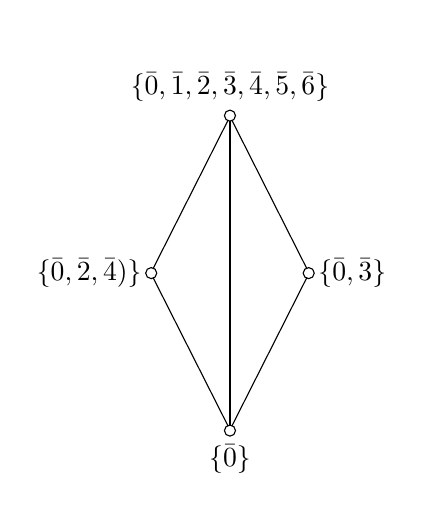
\begin{tikzpicture}
	\draw (0,0)node[left]{$\{\bar{0},\bar{2},\bar{4})\}$}
	(0.025,0.06)--(0.975,1.94);
	\draw (0.025,-0.06)--(0.975,-1.94);
	\draw (1.025,1.94)--(1.975,0.06);
	\draw (1.025,-1.94)--(1.975,-0.06) (2,0)node[right]{$\{\bar{0},\bar{3}\}$};
	\draw (1,-1.93) node[below=3.5pt]{$\{\bar{0}\}$}--(1,1.93) node[above=3.5pt]{$\{\bar{0},\bar{1},\bar{2},\bar{3},\bar{4},\bar{5},\bar{6}\}$} ;
	\draw (0,0) circle [radius=2pt] ;
	\draw (1,2) circle [radius=2pt];
	\draw (1,-2) circle [radius=2pt];
	\draw (2,0) circle [radius=2pt];
	\draw (0,3) node[]{};
	\end{tikzpicture}	
\end{center}

\end{solution}	


\subsection{\textsection7. Quotient groups}
\begin{problem}[7.1]
$\vartriangleright$ List all subgroups of $S_3$ (cf. \hyperlink{Exercise II.6.13}{Exercise II.6.13}) and determine which subgroups are normal and which are not normal. [\textsection7.1]
\end{problem}
\begin{solution}
	The subgroups of $S_3$ are $\{(1)\},\{(1),(12)\},\{(1),(13)\},\{(1),(23)\},\{(1),(123),(132)\}$ and $S_3$. We can check that $\{(1)\},\{(1),(123),(132)\},S_3$ are normal subgroups while others are not.
\end{solution}	

\begin{problem}[7.2]
Is the image of a group homomorphism necessarily a normal subgroup of the target?
\end{problem}
\begin{solution}
No. According to exercise 7.1 we have seen not all subgroups are normal. Suppose $H$ is a subgroup of $G$ but not normal. Then $H$ itself is the image of the inclusion homomorphism $i:H\hookrightarrow G$, which makes a counterexample.   
\end{solution}

\begin{problem}[7.3]
$\vartriangleright$ Verify that the equivalent conditions for normality given in §7.1 are indeed equivalent. [\textsection7.1]
\end{problem}
\begin{solution}
That a subgroup $N$ of $G$ is normal has four equivalent conditions:
\begin{enumerate}
	\item[(i)] $\forall g\in G,\ gNg^{-1}= N$;
	\item[(ii)] $\forall g\in G,\ gNg^{-1}\subseteq N$;
	\item[(iii)] $\forall g\in G,\ gN\subseteq Ng$;
	\item[(iv)] $\forall g\in G,\ gN= Ng$.
\end{enumerate}
(i)$\implies$(ii) is straightforward. \\
(ii)$\implies$(iii). For any $g\in G$, the element $a\in gN$ can be written as $a=gn_1(n_1\in N)$. Since $gn_1g^{-1}\in gNg^{-1}\subseteq N$, there exists an $n_2\in N$ such that $gn_1g^{-1}=n_2$, which implies $gn_1=n_2g\in Ng$. Thus we have $gN\subseteq Ng$.\\	
(iii)$\implies$(iv). Given any $g\in G$, for all $n_1\in N$, the element $g^{-1}n_1\in g^{-1}N_1$ also belongs to $Ng^{-1}$, which implies that there exists $n_2\in N$ such that $g^{-1}n_1=n_2g^{-1}$, namely $n_1g=gn_2$. Thus we get $Ng\subseteq gN$ and accordingly $gN= Ng$.\\
(iv)$\implies$(i). For any $g\in G$, the element $b\in gNg^{-1}$ can be written as $a=gn_1g^{-1}(n_1\in N)$. Since $gn_1\in gN= Ng$, there exists an $n_2\in N$ such that $gn_1=n_2g$, which implies $gn_1g^{-1}=n_2\in N$. Thus we have 
\begin{align*}
	&\forall g\in G,\quad gNg^{-1}\subseteq N\\
	\implies& \forall g^{-1}\in G,\quad g^{-1}(gNg^{-1})g\subseteq gNg^{-1}\\
	\implies& \forall g\in G,\quad N\subseteq gNg^{-1}.
\end{align*}
Hence we have $\forall g\in G,\ gNg^{-1}=N$.
\end{solution}


\begin{problem}[7.4]
Prove that the relation defined in \hyperlink{Exercise II.5.10}{Exercise II.5.10} on a free abelian group $F =F^{ab}(A)$ is compatible with the group structure. Determine the quotient $F/\sim$ as a better known group.
\end{problem}
\begin{solution}
For all $f,f',h\in F$,
\[
f\sim f'\iff f-f'=2g,\,(g\in F)\implies (h+f)-(h+f')=2g,\,(g\in F)\iff h+f\sim h+f'.
\]
Since $F$ is abelian, wee see the relation $\sim$ defined on a free abelian group $F =F^{ab}(A)$ is compatible with the group structure. By the notation of quotient group, we have 
\[
F/\hspace{-2pt}\sim\hspace{4pt}=F/2F,
\]
where $2F=\{2g\in F\,|\,g\in F\}$.
\end{solution}


\begin{problem}[7.5]
$\neg$ Define an equivalence relation $\sim$ on $\SL_2(\Z)$ by letting $A\sim A'\iff A'=\pm A.$ Prove that $\sim$ is compatible with the group structure. The quotient $\SL_2(\Z)/\sim$ is denoted $\mathrm{PSL}_2(\Z)$, and is called the \emph{modular group}; it would be a serious contender in a context for \textquoteleft the most important group in mathematics', due to its role in algebraic geometry and number theory. Prove that $\mathrm{PSL}_2(\Z)$ is generated by the (cosets of the) matrices
\[
\begin{pmatrix}
0 & -1\\
1 & 0\\
\end{pmatrix}
\quad\text{ and }\quad 
\begin{pmatrix}
1 & -1\\
1 & 0\\
\end{pmatrix}.
\]
(You will not need to work very hard, if you use the result of \hyperlink{Exercise 6.10}{Exercise 6.10}.) Note that the first has order 2 in $\mathrm{PSL}_2(\Z)$, the second has order 3, and their product has infinite order. [9.14]
\end{problem}
\begin{solution}
For all $A_1,A_2,B\in \SL_2(\Z)$,
\[
A_1\sim A_2\iff A_2=\pm A_1\iff  BA_2=\pm BA_1\iff BA_1\sim BA_2.
\]	
Hence $\sim$ is compatible with the group structure and $\mathrm{PSL}_2(\Z)=\SL_2(\Z)/\{I_2,-I_2\}$. In \hyperlink{Exercise 6.10}{Exercise 6.10} we have shown $\SL_2(\Z)$ is generated by the matrices
\[
s =
\begin{pmatrix}
0 & -1\\
1 & 0\\
\end{pmatrix}
\quad\text{ and }\quad 
t =
\begin{pmatrix}
1 & 1\\
0 & 1\\
\end{pmatrix}.
\] 
It is clear that $\SL_2(\Z)$ can also be generated by the matrices
\[
s =
\begin{pmatrix}
0 & -1\\
1 & 0\\
\end{pmatrix}
\quad\text{ and }\quad 
ts =
\begin{pmatrix}
1 & -1\\
1 & 0\\
\end{pmatrix},
\] 
which implies $\mathrm{PSL}_2(\Z)$ is generated by the cosets of the matrices $s$ and $ts$.
\end{solution}

\begin{problem}[7.6]
Let $G$ be a group, and let $n$ be a positive integer. Consider the relation
\[
a\sim b\iff(\exists g\in G)ab^{-1}=g^n.
\]
\begin{itemize}
	\item Show that in general $\sim$ is not an equivalence relation.
	\item Prove that $\sim$ is an equivalence relation if $G$ is commutative, and determine the corresponding subgroup of $G$.
\end{itemize}

\end{problem}
\begin{solution}
\begin{itemize}
	\item Let $G$ be the symmetric group $S_4$ and let $n=2$. We can check that
	\begin{align*}
		&(3\ 4)(2\ 3)^{-1}=(2\ 4\ 3)=(2\ 3\ 4)^2\implies(3\ 4)\sim (2\ 3)\\
		&(2\ 3)(1\ 2)^{-1}=(1\ 3\ 2)=(1\ 2\ 3)^2\implies(2\ 3)\sim (1\ 2)
	\end{align*}
	but $(3\ 4)(1\ 2)^{-1}=(1\ 2)(3\ 4)$ is not the square of any element in $S_4$.
	\item Suppose that $G$ is commutative. $aa^{-1}=e^n$ implies $\sim$ is reflexive. Since
	\[
	a\sim b\implies ab^{-1}=g^n\;(g\in G)\implies b^{-1}a=g^{-n}\;(g^{-1}\in G)\implies b\sim a,
	\]  
	$\sim$ is symmetric. Since $G$ is commutative, we have
	\begin{align*}
		&a\sim b,b\sim c\implies ab^{-1}=g_1^n,bc^{-1}=g_2^n\;(g_1,g_2\in G)\\
		\implies& ac^{-1}=ab^{-1}bc^{-1}=g_1^ng_2^n=(g_1g_2)^n\;(g_1g_2\in G)\implies a\sim c,
	\end{align*}
	which means $\sim$ is transitive. Thus we show that $\sim$ is an equivalence relation. Since
	\[
	a\sim b\implies ab^{-1}=g^n\implies ga(gb)^{-1}=(ag)(bg)^{-1}=g^n\implies ga\sim gb,ag\sim bg,
	\]
	we see $\sim$ is compatible with the group $G$ and the equivalence class of the identity $H=\{g^n|g\in G\}$ is a subgroup of $G$.
\end{itemize}
\end{solution}

\begin{problem}[7.7]
	Let $G$ be a group, $n$ a positive integer, and let $H \subseteq G$ be the subgroup
	generated by all elements of order $n$ in $G$. Prove that $H$ is normal.
\end{problem}
\begin{solution}
	For all $h\in H, g\in G$, we have 
	$$(ghg^{-1})^n=gh^ng^{-1}=gg^{-1}=e_G\implies ghg^{-1}\in H,  $$
	which means $gHg^{-1}\subseteq H$ for all $g\in G$. Thus we show that $H$ is normal.
\end{solution}

\begin{problem}[7.10]
$\neg$ Let $G$ be a group, and $H\subseteq G$ a subgroup. With notation as in \hyperlink{Exercise II.6.7}{Exercise II.6.7}, show that $H$ is normal in $G$ if and only if $\forall \gamma \in \Inn(G), \gamma(H) \subseteq H$.
Conclude that if $H$ is normal in $G$ then there is an interesting homomorphism
$\Inn(G)\to \Aut(H)$. [8.25]
\end{problem}
\begin{solution}
Consistent with the notation as in \hyperlink{Exercise II.6.7}{Exercise II.6.7}, suppose
\[
\gamma_g:G\longrightarrow G,\ h\longmapsto ghg^{-1}.
\]
Then we have
\[
\forall \gamma_g \in \Inn(G), \gamma_g(H) \subseteq H\iff \forall g\in G, gHg^{-1}\subseteq H\iff \text{$H$ is normal in $G$}.
\]
Thus we see that if $H$ is normal in $G$, $\gamma$ can be restricted to $H$ so that $\gamma|_H:H\rightarrow H$ is an automorphism on $H$. Let 
\[
i:\Inn(G)\longrightarrow \Aut(H),\ \gamma\longmapsto\gamma|_h
\]
and with the property of $\gamma$ we have shown in \hyperlink{Exercise II.4.8}{Exercise II.4.8}, it is straightforward to check that
\[
i(\gamma_{g_1}\gamma_{g_2})=i(\gamma_{g_1g_2})=\gamma_{g_1g_2}|_h=(\gamma_{g_1}\gamma_{g_2})|_h=\gamma_{g_1}|_h\gamma_{g_2}|_h=i(\gamma_{g_1})i(\gamma_{g_2}).
\]
That is, $i$ is the interest homomorphism $\Inn(G)\to \Aut(H)$ that we expect.
\end{solution}

\hypertarget{Exercise II.7.11}{}
\begin{problem}[7.11]
$\vartriangleright$ Let $G$ be a group, and let $[G,G]$ be the subgroup of $G$ generated by all elements of the form $aba^{-1}b^{-1}$. (This is the commutator subgroup of $G$; we will return to it in \textsection IV.3.3.) Prove that $[G,G]$ is normal in $G$. (Hint: with notations in \hyperlink{Exercise II.4.8}{Exercise II.4.8}, $gaba^{-1}b^{-1}g^{-1} = \gamma_g(aba^{-1}b^{-1})$.) Prove that $[G,G]$ is normal in $G$. [7.12, \textsection IV.3.3]
\end{problem}
\begin{solution}
Since for all $g\in G, aba^{-1}b^{-1}\in[G,G]$, we have
\[
gaba^{-1}b^{-1}g^{-1}=gag^{-1}gbg^{-1}ga^{-1}g^{-1}gb^{-1}g^{-1}=(gag^{-1})(gbg^{-1})(gag^{-1})^{-1}(gbg^{-1})^{-1}\in[G,G],
\]
it follows that that $[G,G]$ is normal in $G$. Then we can show $[G,G]$ is normal in $G$ by
\[
[g_1][g_2]=[g_1g_2]=[g_1g_2(g_2^{-1}g_1^{-1}g_2g_1)]=[g_2g_1]=[g_2][g_1],\quad\forall [g_1],[g_2]\in[G,G].
\]
\end{solution}

\hypertarget{Exercise II.7.12}{}
\begin{problem}[7.12]
$\vartriangleright$ Let $F = F(A)$ be a free group, and let $f : A\to G$ be a set-function
from the set $A$ to a commutative group $G$. Prove that $f$ induces a unique homomorphism $F/[F, F]\to G$, where $[F, F]$ is the commutator subgroup of $F$ defined in \hyperlink{Exercise II.7.11}{Exercise II.7.11}. (Use Theorem 7.12.) Conclude that $F/[F, F]\simeq F^{ab}(A)$. (Use Proposition I.5.4.) [\textsection6.4, 7.13, VI.1.20]
\end{problem}
\begin{solution}
By the universal property of free group, there exists a unique homomorphism $\varphi:F\to G$ such that $\forall a\in A,\;\varphi(j(a))=f(a)$ 
where $j:A\to F(A)$ is a inclusion. Note that $G$ is commutative, we have
\[
\varphi(aba^{-1}b^{-1})=\varphi(a)\varphi(b)\varphi(a)^{-1}\varphi(b)^{-1}=e_G,
\]
which implies $[F,F]\subseteq \ker\varphi$. Theorem 7.12 indicates that there exists a unique group homomorphism $\tilde{\varphi}:F/[F, F]\to G$ so that $\tilde{\varphi}\circ\pi=\varphi$. Now we deduce that the diagram
\[\xymatrix{
	A\ar@{->}[d]_{j}\ar@{->}[rd]^{f} \\
	F\ar@{->}[r]^{\exists!\varphi}\ar@{->}[d]_{\pi} & G\\
	F/[F,F]\ar@{->}[ru]_{\exists!\tilde{\varphi}}  
}\]
commutes. For the diagram we see $\tilde{\varphi}\circ\pi\circ j=f$. Suppose there exists $\psi$ such that $\psi\circ\pi\circ j=f$, which amounts to $(\psi\circ\pi)\circ j=\varphi\circ j$. By the uniqueness of $\varphi$ we have $\psi\circ\pi=\varphi$. Then by the uniqueness of $\tilde{\varphi}$ we have $\psi=\tilde{\varphi}$. Thus we show that there exists unique $\tilde{\varphi}$ such that $\tilde{\varphi}\circ\pi\circ j=f$. According to the property of free abelian group, we can conclude that $F/[F, F]\simeq F^{ab}(A)$.
\end{solution}

\begin{problem}[7.13]
$\neg$ Let $A, B$ be sets, and $F(A), F(B)$ the corresponding free groups. Assume $F(A)\simeq F(B)$. If $A$ is finite, prove that so is $B$, and $A\simeq B$. (Use \hyperlink{Exercise II.7.12}{Exercise II.7.12} to upgrade \hyperlink{Exercise II.5.10}{Exercise II.5.10}.) [5.10, VI.1.20]
\end{problem}
\begin{solution}
\hyperlink{Exercise II.7.12}{Exercise II.7.12} tells us that the free abelian group generated by a set is merely determined by its free group, which means
\[
F(A)\simeq F(B)\implies F(A)/[F(A),F(A)]\simeq F(B)/[F(B),F(B)]\implies F^{ab}(B)\cong F^{ab}(A).
\]
Then under the auspices of the conclusion in \hyperlink{Exercise II.5.10}{Exercise II.5.10} we complete the proof.
\end{solution}


\subsection{\textsection8. Canonical decomposition and Lagrange's theorem}
\begin{problem}[8.1]
	If a group $H$ may be realized as a subgroup of two groups $G_1$ and $G_2$, and
\[
	\frac{G_1}{H}\cong \frac{G_2}{H},
\]
does it follows that $G_1\cong G_2$. Give a proof or a counterexample.
\end{problem}
\begin{solution}
	A counterexample is given as follows. Take $H=C_3$, the cyclic group of order $3$. Take $G_1=D_6$ and $G_2=C_6$, then one sees both $G_1/H$ and  $G_2/H$ are $C_2$. But obviously $G_1$ and $G_2$ are not isomorphic, one being abelian while the other is not.
\end{solution}

\begin{problem}[8.2]
$\neg$ Extend Example 8.6 as follows. Suppose $G$ is a group, and $H\subseteq G$ is a subgroup of index 2: that is, such that there are precisely two (say, left) cosets of $H$ in $G$. Prove that $H$ is normal in $G$. [9.11, IV.1.16]
\end{problem}
\begin{solution}
Since $[G/H]=2$, there must be $G/H=\{H,G-H\}$. For any $g\in G	$: 
\begin{itemize}
	\item if $g\in H$, then $gH=Hg=H$;
	\item if $g\in G-H$, then $gH\ne H$ and $Hg\ne H$. Thus we have $gH=Hg=G-H$.
\end{itemize}
In either case $gH=Hg$ holds for all $g\in G$, which implies $H$ is normal in $G$.
\end{solution}

\begin{problem}[8.7]
Let $(A|\mathscr{R})$, resp. $(A'|\mathscr{R}')$ be presentations for two groups $G$, resp. $G'$(cf. §8.2); we may assume that $A, A'$ are disjoint. Prove that the group $G*G'$ presented by
\[
(A\cup A'|\mathscr{R}\cup \mathscr{R}')
\]
satisfies the universal property for the \emph{coproduct} of $G$ and $G'$ in $\Grp$. (Use the universal properties of both free groups and quotients to construct natural homomorphisms $G\to G*G'$, $G'\to G* G'$.) [\textsection3.4, \textsection8.2, 9.14].
\end{problem}
\begin{solution}
Assume that $F(A)/R=(A|\mathscr{R})$, $F(A')/R'=(A|\mathscr{R}')$, and $F(A\amalg A')/R''=(A\cup A'|\mathscr{R}\cup \mathscr{R}')$.
	\[\xymatrix{
		&G&\\
		F(A)/R\ar[ru]^{f}\ar@{-->}[r]^{\psi\hspace{1em}}&F(A\amalg A')/R''\ar@{-->}[u]^{\delta}&F(A')/R'\ar[lu]_{f'}\ar@{-->}[l]_{\hspace{1em}\psi'}\\
		A\ar[rd]_{i}\ar[u]^{k}&F(A\amalg A')\ar[u]_{\pi}&A'\ar[ld]^{i'}\ar[u]_{k'}\\
		&A\amalg A'\ar[u]_{j} &
	}\]
According to \hyperlink{Lemma II.1}{Lemma II.1}, there exist unique $\psi$ and $\psi'$ such that 
\[
\psi\circ k=\pi\circ j\circ i,\ \psi'\circ k'=\pi\circ j\circ i'.
\]
Define 
\begin{align*}
\delta:&F(A\amalg A')/R''\longrightarrow G\\
&[\{a_1\}*\{a_1'\}*\cdots*\{a_n\}*\{a_n'\}]\longmapsto f([\{a_1\}])f'([\{a_1'\}])\cdots f([\{a_n\}])f'([\{a_n'\}]).
\end{align*}
where $*$ means the junction of words and $\{a_i\}=a_{i1}*a_{i2}*\cdots *a_{im_i}$, $a_{ij}\in A$ $(1\le i\le n,1\le j\le m_i)$ and $\{a_i'\}=a_{i1}'*a_{i2}'*\cdots *a_{im_i'}$, $a_{ij'}\in A$ $(1\le i\le n,1\le j'\le m_i')$.
It is routine to check that $\delta$ is a well-defined homomorphism such that 
$$
\delta\circ\psi=f,\ \delta\circ\psi'=f'.
$$ 
Then verify that if $\hat{\delta}$ is a homomorphism such that 
$$
\delta\circ\psi=f,\ \delta\circ\psi'=f',
$$ 
there must be $\hat{\delta}=\delta$. After these tasks are done, we can conclude that $F(A\amalg A')/R''$ satisfies the universal property of coproduct.

\end{solution}

\subsection{\textsection9. Group actions}

\subsection{\textsection10. Group objects in categories}

\section{Chapter III\quad Chapter Rings and modules}

\subsection{\textsection1. Definition of ring}
\begin{problem}[1.1]
	$\vartriangleright$ Prove that if $0 = 1$ in a ring $R$, then $R$ is a zero-ring. [\textsection1.2]
\end{problem}
\begin{solution}
	For any $x$ in the ring $R$, we have
	\[
	1\cdot x=x,\qquad 0\cdot x=0.
	\]
	Since $0 = 1$ we see that $x=0$, which implies $R$ is a ring with only one element $0$.
\end{solution}

\begin{problem}[1.2]
	$\neg$ Let $S$ be a set, and define operations on the power set $\mathscr{P}(S)$ of $S$ by setting $\forall A,B \in \mathscr{P}(S)$
	\[
	A+B :=(A \cup B) \backslash(A \cap B) \quad, \quad A \cdot B=A \cap B
	\]
	Prove that $(\mathscr{P}(S),+,\cdot)$ is a commutative ring. [2.3, 3.15]
\end{problem}
\begin{solution}
	First, we need to check that $(\mathscr{P}(S),+)$ is an abelian group:
	\begin{itemize}
		\item associativity:	
		\begin{align*}
		&\hspace{1em}(A+B)+C\\
		&=((A \cup B) \backslash(A \cap B))+C\\
	    &=((A \cup B) \cap(A^C \cup B^C))+C\\
	    &=(A\cap(A^C \cup B^C) )\cup (B\cap(A^C \cup B^C)) +C\\
	    &=(A \cap B^C) \cup(A^C \cap B)+C\\
	    &=(((A \cap B^C) \cup(A^C \cap B)) \cap C^C) \cup(((A \cap B^C) \cup(A^C \cap B))^C \cap C)\\
	    &=((A \cap B^C\cap C^C )\cup(A^C \cap B\cap C^C) ) \cup((A^C \cup B) \cap(A\cup B^C)\cap C)\\
	    &=((A \cap B^C\cap C^C )\cup(A^C \cap B\cap C^C) ) \cup((A^C\cap B^C) \cup( A\cap B) \cap C)\\
	    &=(A \cap B^C\cap C^C )\cup(A^C \cap B\cap C^C)  \cup(A^C\cap B^C\cap C) \cup( A\cap B\cap C) \\
	    &=(A \cap (B \cap C) \cup(B^C \cap C^C)) \cup((A^C \cap B \cap C^C) \cup (A^C \cap B^C \cap C))\\
	    &=(A \cap (B^C \cup C) \cap(B \cup C^C)) \cup((A^C \cap B \cap C^C) \cup (A^C \cap B^C \cap C))\\
	    &=(A \cap ((B \cap C^C) \cup(B^C \cap C))^C) \cup(A^C \cap ((B \cap C^C) \cup(B^C \cap C)))\\
	    &=A+((B \cap C^C) \cup(B^C \cap C))\\
	    &=A+(B+C);
		\end{align*}
		\item commutativity:
		\[
		A+B =(A \cup B) \backslash(A \cap B)=(B \cup A) \backslash(B \cap A)= B+A;
		\]
		\item additive identity: the additive identity is $\varnothing$ since
		\[
		A+\varnothing=(A \cup \varnothing) \backslash(A \cap \varnothing)=A; \backslash\varnothing=A
		\] 
		\item inverse: the inverse of some set $A$ is just itself since
		\[
		A+A=(A \cup A) \backslash(A \cap A)=A\backslash A=\varnothing.
		\]
	\end{itemize}
	Then we have to show that $(\mathscr{P}(S),\cdot)$ is a commutative monoid, which clearly holds with the multiplicative identity $S$. What is left to show is the distributive properties and the check is straightforward.
	\begin{align*}
	&\hspace{1em}(A+B)\cdot C\\
	&=((A \cap B^C) \cup(A^C \cap B))\cap C\\
	&=(A \cap B^C\cap C) \cup(A^C \cap B\cap C)\\
	&=(A\cap C \cap (B^C\cup C^C)) \cup((A^C\cup C^C) \cap (B\cap C))\\
	&=(A\cap C \cap (B\cap C)^C) \cup((A\cap C)^C \cap (B\cap C))\\
	&=A\cdot C+B\cdot C.
	\end{align*}
\end{solution}

\begin{problem}[1.3]
	$\neg$ Let $R$ be a ring, and let $S$ be any set. Explain how to endow the set $R^S$ of set-functions $S\to R$ of two operations $+$, $\cdot$ so as to make $R^S$ into a ring, such that $R^S$ is just a copy of $R$ if $S$ is a sigleton. [2.3]
\end{problem}
\begin{solution}
	To make $(R^S,+,\cdot )$ a ring , for all $f,g\in R^S$ we define addition and multiplication as
	\begin{align*}
	f+g&:S\longrightarrow R,\quad x\longmapsto f(x)+g(x)\\
	f\cdot g&:S\longrightarrow R,\quad x\longmapsto f(x)\cdot g(x).
	\end{align*}
\end{solution}

\begin{problem}[1.4]
	$\vartriangleright$ The set of $n\times n$ matrices with entries in a ring $R$ isdenoted $\mathcal{M}_n(R)$. Prove that componentwise addition and matrixmultiplication makes $\mathcal{M}_n(R)$ into a ring, for any ring $R$. The notation $\mathfrak{gl}_n(R)$ is also commonly used, especially $R=\mathbb{R}$ or $\mathbb{C}$ (although this indicates one is considering them as \emph{Lie algebras}) in parallel with the analogous notation for the corresponding groups of units, cf. \hyperlink{Exercise II.6.1}{Exercise II.6.1}. In
	fact, the parallel continues with the definition of the following sets of matrices:
	\begin{itemize}
		\item $\mathfrak{sl}_n(\mathbb{R}) = \{M \in \mathfrak{gl}_n(\mathbb{R}) | \mathrm{tr}(M) = 0\}$;
		\item $\mathfrak{sl}_n(\mathbb{C}) = \{M \in \mathfrak{gl}_n(\mathbb{C}) | \mathrm{tr}(M) = 0\}$;
		\item $\mathfrak{so}_n(\mathbb{R}) = \{M \in \mathfrak{sl}_n(\mathbb{R}) |M +M^t = 0\}$;
		\item $\mathfrak{su}_n(\mathbb{C}) = \{M \in \mathfrak{sl}_n(\mathbb{C}) |M +M^\dag = 0\}$.
	\end{itemize}
	Here $\mathrm{tr}(M)$ is the trace of $M$, that is, the sum of its diagonal entries. The other notation matches the notation used in Exercise II.6.1. Can we make rings of these sets, by endowing them of ordinary addition and multiplication of matrices? (These sets are all Lie algebras, cf. Exercise VI.1.4.) [\textsection1.2, 2.4, 5.9, VI.1.2, VI.1.4]
\end{problem}
\begin{solution}
	It is plain to show $\mathcal{M}_n(R)$ is a ring according to the definition. For multiplicative associativity, it follows that for all $A,B,C\in\mathcal{M}_n(R)$,
	\begin{align*}
	&\hspace{1em}((A B) C)_{\alpha, \delta}\\
	&=\sum_{i=1}^{n}(A B)_{\alpha, i} c_{i, \delta}\\
	&=\sum_{i=1}^{n}\left(\sum_{j=1}^{n} a_{\alpha, j} b_{j, i}\right) c_{i, \delta}\\
	&=\sum_{i=1}^{n} \sum_{j=1}^{n}\left(a_{\alpha, j} b_{j, i}\right) c_{i, \delta}\\
	&=\sum_{j=1}^{n} \sum_{n=1}^{n} a_{\alpha, j}\left(b_{j, i} c_{i, \delta}\right)\\
	&=\sum_{j=1}^{n} a_{\alpha, j}\left(\sum_{i=1}^{n} b_{j, i} c_{i, \delta}\right)\\
	&=\sum_{j=1}^{n} a_{\alpha, j}(B C)_{j, \delta}\\
	&=(A(B C))_{\alpha, \delta}.
	\end{align*}
	Under the ordinary addition and multiplication of matrices, $\mathfrak{sl}_n(\mathbb{R}),\mathfrak{sl}_n(\mathbb{C}),\mathfrak{so}_n(\mathbb{R}),\mathfrak{su}_n(\mathbb{C})$ are not rings. In fact, they are not closed under the multiplication.
\end{solution} 

\begin{problem}[1.5]
	Let $R$ be a ring. If $a, b$ are zero-divisors in $R$, is $a+b$ necessarily a zero-divisor?
\end{problem}
\begin{solution}
	That is not true. Let's take $\mathbb{Z}/6\mathbb{Z}$ as an counterexample. Though both $[2]_6$ and $[3]_6$ are zero-divisors, their sum $[5]_6$ is not a zero-divisor.
\end{solution}

\begin{problem}[1.6]
	$\neg$ An element $a$ of a ring $R$ is \emph{nilpotent} if $a^n = 0$ for some $n$.
	\begin{enumerate}
	\item Prove that if $a$ and $b$ are nilpotent in $R$ and $ab = ba$, then $a+b$ is also nilpotent.
	\item Is the hypothesis $ab = ba$ in the previous statement necessary for its conclusion to hold?
	\end{enumerate}
[3.12]
\end{problem}
\begin{solution}
	\begin{enumerate}
		\item Assume that $a^n=b^m=0$ and let $k=2\max\{n,m\}$. If $ab = ba$, we can get
		\[
		(a+b)^k=\sum_{p=0}^{\tfrac{k}{2}}\binom{k}{p}a^kb^{k-p}+\sum_{p=\tfrac{k}{2}+1}^{k}\binom{k}{p}a^kb^{k-p}=\sum_{p=0}^{\tfrac{k}{2}}\binom{k}{p}a^k\cdot 0+\sum_{p=\tfrac{k}{2}+1}^{k}\binom{k}{p}0\cdot b^{k-p}=0,
		\]
		which means $a+b$ is also nilpotent.
		\item The hypothesis $ab = ba$ is necessary. A counterexample can be found in the ring $\mathfrak{gl}_2(\mathbb{R})$. Let
		\[
		a=\left(
		\begin{matrix}	
		0 & 1\\	
		0 & 0	
		\end{matrix}
		\right),\quad
		b=\left(
		\begin{matrix}	
		0 & 0\\	
		1 & 0	
		\end{matrix}
		\right)
		\]
		and then we have $a^2=b^2=0$. In other words, $a$ and $b$ are nilpotent. However, by diagonalization we see that
		\[
		(a+b)^n=
		\left(
		\begin{matrix}	
		0 & 1\\	
		1 & 0	
		\end{matrix}
		\right)^n
		=\left(
		\begin{matrix}	
		-1 & 1\\	
		1 & 1	
		\end{matrix}
		\right)
		\left(
		\begin{matrix}	
		-1 & 0\\	
		0 & 1	
		\end{matrix}
		\right)^n
		\left(
		\begin{matrix}	
		-1 & 1\\	
		1 & 1	
		\end{matrix}
		\right)^{-1}\ne 
		\left(
		\begin{matrix}	
		0 & 0\\	
		0 & 0	
		\end{matrix}
		\right).
		\]
		Thus in such case, $a+b$ is no longer nilpotent.
	\end{enumerate}
\end{solution}

\begin{problem}[1.8]
	Prove that $x = \pm1$ are the only solutions to the equation $x^2 = 1$ in an integral	domain. Find a ring in which the equation $x^2 = 1$ has more than 2 solutions.
\end{problem}
\begin{solution}
	It clearly holds that $1\cdot1=1$ and $(-1)\cdot(-1)=((-1)\times(-1))1\cdot1=1$. That is to say,  $x = \pm1$ are the solutions to the equation $x^2 = 1$. Note that if there exists $x$ in an integral	domain such that $x^2=1$, then we have
	\[
	(x-1)\cdot(x+1)=x^2-1=0,
	\]
	which implies $x-1=0$ or $x+1=0$. Therefore, we can assert $x = \pm1$ are the solutions. In the ring $\mathbb{Z}/8\mathbb{Z}$, $[3]_8$ and $[5]_8$ are also the solutions to the equation $x^2 = 1$.
\end{solution}

\begin{problem}[1.10]
	Let $R$ be a ring. Prove that if $a \in R$ is a right unit, and has two or more left-inverses, then $a$ is not a left-zero-divisor, and is a right-zero-divisor.
\end{problem}
\begin{solution}
	Since $a \in R$ is a right unit, it cannot be a left-zero-divisor. Assume there exist two distinct elements $x,y\in R$ such that $xa=ya=1$ and it deduces $(y-x)a=0$. Thus we show that $a$ a right-zero-divisor.
\end{solution}

\begin{problem}[1.11]
	Construct a field with 4 elements: as mentioned in the text, the underlying
	abelian group will have to be $\mathbb{Z}/2\mathbb{Z}\times\mathbb{Z}/2\mathbb{Z}$; $(0, 0)$ will be the zero element, and (1, 1) will be the multiplicative identity. The question is what $(0, 1)\cdot(0, 1)$, $(0, 1)\cdot(1, 0)$, $(1, 0)\cdot(1, 0)$ must be, in order to get a field. [\textsection1.2, \textsection V.5.1]
\end{problem}
\begin{solution}
	Define 
	\[
	(0, 1)\cdot(0, 1)=(0, 1),\quad (0, 1)\cdot(1, 0)=(0,0),\quad (1, 0)\cdot(1, 0)=(1, 0),
	\]
	and the the rest definition of multiplication will be determined uniquely according to field properties. For example, we have no alternatives but to define
	\[
	(0, 1)\cdot(1,1)=(0, 1)\cdot((0,1)+(1,0))=(0, 1)\cdot(0,1)+(0, 1)\cdot(1,0)=(0, 1)+(0,0)=(0,1).
	\]
	Then we can check $\mathbb{Z}/2\mathbb{Z}\times\mathbb{Z}/2\mathbb{Z}$ forms a field by definition. 
\end{solution}

\begin{problem}[1.12]
	Just as complex numbers may be viewed as combinations $a+bi$, where
	$a,b\in \R$, and $i$ satisfies the relation $i^2=-1$ (and commutes with $\R$), we may construct a ring $\mathbb{H}$ by considering linear combinations $a + bi + cj + dk$ where $a, b, c, d \in \R$, and $i, j, k$ commute with $\R$ and satisfy the following relations:
	\[
	i^{2}=j^{2}=k^{2}=-1 \quad, \quad i j=-j i=k \quad, \quad j k=-k j=i \quad, \quad k i=-i k=j.
	\]
	Addition in $\mathbb{H}$ is defined componentwise, while multiplication is defined by imposing	distributivity and applying the relations. For example,
	\[
	(1+i+j) \cdot(2+k)=1 \cdot 2+i \cdot 2+j \cdot 2+1 \cdot k+i \cdot k+j \cdot k=2+2 i+2 j+k-j+i=2+3 i+j+k.
	\]
	\begin{enumerate}[(i)]
		\item Verify that this prescription does indeed define a ring.
		\item Compute $(a+b i+c j+d k)(a-b i-c j-d k)$, where $a, b, c, d \in \R$.
		\item Prove that $\mathbb{H}$ is a division ring. Elements of $\mathbb{H}$ are called quaternions. Note that $Q_8 := \{\pm1,\pm i,\pm j,\pm k\}$ forms a subgroup of the group of units of $\mathbb{H}$; it is a noncommutative group of order 8, called the quaternionic group.
		\item  List all subgroups of $Q_8$, and prove that they are all normal.
		\item  Prove that $Q_8$, $D_8$ are not isomorphic.
		\item  Prove that $Q_8$ admits the presentation $\left(x, y | x^{2} y^{-2}, y^{4}, x y x^{-1} y\right)$.
	\end{enumerate}
	[\textsection II.7.1, 2.4, IV.1.12, IV.5.16, IV.5.17, V.6.19]
\end{problem}
\begin{solution}
	\begin{enumerate}[(i)]
		\item Verifying the $(\mathbb{H},+)$ is a abelian group is immediate and we just omitted it. It is easy to see the multiplicative identity is 1 and the distributive properties are guaranteed by definition. The check of the associativity of multiplication looks straightforward but tedious.
		\begin{align*}
			&\hspace{1.2em}((a_1+b_1i+c_1j+d_1k)\cdot(a_2+b_2i+c_2j+d_2k))\cdot(a_3+b_3i+c_3j+d_3k)\\
			&=[-c_3 \left(a_ 2 c_ 1+a_ 1 c_ 2+b_ 2 d_ 1-b_ 1 d_ 2\right)-b_ 3
			\left(a_ 2 b_ 1+a_ 1 b_ 2-c_ 2 d_ 1+c_ 1 d_ 2\right)\\
			&\hspace{1em}+a_ 3 \left(a_ 1a_ 2-b_ 1b_ 2-c_ 1 c_ 2-d_ 1 d_ 2\right)-d_3\left(-b_2 c_ 1+b_ 1 c_ 2+a_ 2 d_1+a_ 1 d_ 2\right)  ]\\
			&\hspace{1em}+[-c_3 \left(-b_2 c_ 1+b_ 1 c_ 2+a_ 2 d_ 1+a_ 1 d_ 2\right)+a_ 3 \left(a_ 2 b_ 1+a_ 1
			b_ 2-c_ 2 d_ 1+c_ 1 d_ 2\right)\\
			&\hspace{1em}+b_ 3 \left(a_ 1 a_ 2-b_ 1 b_ 2-c_ 1 c_ 2-d_ 1 d_ 2\right)+d_ 3\left(a_ 2 c_ 1+a_ 1 c_ 2+b_ 2 d_ 1-b_ 1 d_ 2\right) ]i\\
			&\hspace{1em}+[b_ 3 \left(-b_2 c_ 1+b_ 1
			c_ 2+a_ 2 d_ 1+a_ 1 d_ 2\right)+a_ 3 \left(a_ 2 c_ 1+a_ 1 c_ 2+b_ 2d_ 1-b_ 1 d_ 2\right)\\
			&\hspace{1em}+c_ 3 \left(a_ 1 a_ 2-b_ 1 b_ 2-c_ 1 c_ 2-d_1d_2\right)-d_ 3\left(a_ 2 b_ 1+a_ 1 b_ 2-c_ 2d_ 1+c_ 1 d_ 2\right) ]j\\
			&\hspace{1em}+[a_ 3 \left(-b_2 c_ 1+b_ 1 c_ 2+a_ 2 d_ 1+a_ 1 d_ 2\right)-b_ 3 \left(a_ 2 c_ 1+a_ 1 c_ 2+b_ 2 d_ 1-b_ 1 d_ 2\right)\\
			&\hspace{1em}+c_ 3 \left(a_2b_ 1+a_ 1 b_ 2-c_ 2d_ 1+c_ 1 d_ 2\right)+d_ 3\left(a_ 1 a_ 2-b_ 1 b_ 2-c_ 1 c_ 2-d_ 1 d_ 2\right) ]k
		\end{align*}
		\begin{align*}
		&\hspace{1.2em}(a_1+b_1i+c_1j+d_1k)\cdot((a_2+b_2i+c_2j+d_2k)\cdot(a_3+b_3i+c_3j+d_3k))\\
		&=[-d_1 \left(a_3 d_2+a_2 d_3-b_3
		c_2+b_2 c_3\right)-c_1 \left(a_3 c_2+a_2 c_3+b_3 d_2-b_2
		d_3\right)\\
		&\hspace{1em}-b_1 \left(a_3 b_2+a_2 b_3-c_3 d_2+c_2
		d_3\right)+a_1 \left(a_2 a_3-b_2 b_3-c_2 c_3-d_2
		d_3\right) ]\\
		&\hspace{1em}+[c_1 \left(a_3 d_2+a_2 d_3-b_3 c_2+b_2
		c_3\right)-d_1 \left(a_3 c_2+a_2 c_3+b_3 d_2-b_2
		d_3\right)\\
		&\hspace{1em}+a_1 \left(a_3 b_2+a_2 b_3-c_3 d_2+c_2
		d_3\right)+b_1 \left(a_2 a_3-b_2 b_3-c_2 c_3-d_2
		d_3\right) ]i\\
		&\hspace{1em}+[-b_1 \left(a_3 d_2+a_2 d_3-b_3 c_2+b_2
		c_3\right)+a_1 \left(a_3 c_2+a_2 c_3+b_3 d_2-b_2
		d_3\right)\\
		&\hspace{1em}+d_1 \left(a_3 b_2+a_2 b_3-c_3 d_2+c_2
		d_3\right)+c_1 \left(a_2 a_3-b_2 b_3-c_2 c_3-d_2
		d_3\right)]j\\
		&\hspace{1em}+[a_1 \left(a_3 d_2+a_2 d_3-b_3 c_2+b_2
		c_3\right)+b_1 \left(a_3 c_2+a_2 c_3+b_3 d_2-b_2
		d_3\right)\\
		&\hspace{1em}-c_1 \left(a_3 b_2+a_2 b_3-c_3 d_2+c_2
		d_3\right)+d_1 \left(a_2 a_3-b_2 b_3-c_2 c_3-d_2
		d_3\right) ]k
		\end{align*}
		\item Expand it by distributive properties and we get
		\begin{align*}
			&(a+b i+c j+d k)(a-b i-c j-d k)\\
			&=a^2-abi-acj-adk+abi+b^2-bck+bdj+acj+bck+c^2-cdi+adk-bdj+cdi+d^2\\
			&=a^2+b^2+c^2+d^2.
		\end{align*}
		\item Applying the results in (ii) we see that for any non-zero element $a+b i+c j+d k\in\mathbb{H}$,
		\[
		(a+b i+c j+d k)\cdot\frac{a-b i-c j-d k}{a^2+b^2+c^2+d^2}=\frac{a-b i-c j-d k}{a^2+b^2+c^2+d^2}\cdot(a+b i+c j+d k)=1,
		\]
		which implies $a+b i+c j+d k$ is a two-sided unit. Thus we show that $\mathbb{H}$ is a division ring. 
		\item $Q_8$ has 6 subgroups: $\{1\}$, $\{1,-1\}$, $\{1,-1,i,-i\}$, $\{1,-1,j,-j\}$, $\{1,-1,k,-k\}$, $Q_8$. We can just prove that they are all normal by the definition of normal subgroups.
		\item Note that $D_8=\{e,r,r^2,r^3,s_1,s_2,s_3,s_4\}$ has 7 subgroups: $\{e\}$, $\{e,r,r^2,r^3\}$, $\{e,s_1\}$, $\{e,s_2\}$, $\{e,s_3\}$, $\{e,s_4\}$, $D_8$, while $Q_8$ has 6 subgroups. Thus $Q_8$, $D_8$ are not isomorphic.
		\item 	Let $P=\left(x, y | x^{2} y^{-2}, y^{4}, x y x^{-1} y\right)$. The relation $x^{2} y^{-2}=e$ implies $x^2=y^2$ and the relation $xyx^{-1}y=e$ implies $yx=yx^{-1}x^2=x^{-1}y^{-1}x^2=x^3y^3x^2=x^3y^5=x^3y$. First, we can always replace $yx$ by $x^3y$ until we obtain a word of the form $x^iy^j$. Then applying $x^4=y^4=e$ and replace $y^2$ by $x^2$, we can transform it into the form $x^iy^j$ with $0\le i\le 3$ and $0\le j \le 1$. Thus we see $P$ has at most 8 elements. 
		
		Next we will complete our proof by means of the \hyperlink{Lemma II.1}{Lemma II.1} in the appendix. Define a mapping
		\begin{align*}
		f:\{x,y\}\longrightarrow Q_8,\quad& x\longmapsto i,\\
		& y\longmapsto j.
		\end{align*}
		Let $\varphi:F(\{x,y\})\to Q_8$ be the unique homomorphism induced by the universal property of free group. Since
		\begin{align*}
		&\varphi(x^{2} y^{-2})=i^2j^{-2}=1,\\
		&\varphi(y^{4})=j^{4}=1,\\
		&\varphi(x y x^{-1} y)=i j i^{-1} j=1,
		\end{align*}
		we see $\mathscr{R}=\{x^{2} y^{-2}, y^{4}, x y x^{-1} y\}\subset\ker\varphi$. And it is immediate to show that $Q_8$ can be generated by $\{i,j\}$. Thus according to the lemma, there exists a unique homomorphism $\psi:P\to Q_8$ such that $f=\psi\circ\pi\circ i$ and actually $\psi$ is surjective. 
		\[\xymatrix{
			P\ar@{-->}[rd]^{\exists!\psi}\\
			F(\{x,y\})\ar@{-->}[r]^{\varphi}\ar[u]^{\pi} &Q_8\\
			\{x,y\}\ar[ru]_{f}\ar[u]^{i}&    
		}\]
		Hence we get the inequality of cardinality $|P|\ge|Q_8|$. Since we have shown $|P|\le 8=|Q_8|$, there must be $|P|=|Q_8|=8$, which implies $\psi$ is indeed an isomorphism. Finally we conclude that $Q_8\cong\left(x, y | x^{2} y^{-2}, y^{4}, x y x^{-1} y\right)$ and complete our proof. 
	
	\end{enumerate}
\end{solution}


\hypertarget{Exercise III.1.14}{}
\begin{problem}[1.14]
	$\vartriangleright$ Let $R$ be a ring, and let $f(x),g(x)\in R[x]$ be nonzero polynomials. Prove that 
	\[
	\deg(f(x) + g(x))\le\max(\deg(f(x)), \deg(g(x))).
	\]
	Assuming that $R$ is an integral domain, prove that	
	\[
	\deg(f(x)\cdot g(x)) = \deg(f(x)) + \deg(g(x)).
	\] 
	[\textsection1.3]
\end{problem}
\begin{solution}
	Assume
	\[
	f(x)=\sum_{i \ge 0} a_{i} x^{i},\quad g(x)=\sum_{i \ge 0} b_{i} x^{i}, \quad a_i,b_i\in R
	\]
	and $n,m$ are respectively the
	largest integers $p,q$ for which $a_p$, $b_q$ are non-zero. In others words, we have $a_n\ne 0$, $a_i=0$ for $i>n$ and $b_m\ne 0$, $b_i=0$ for $i>m$. Since
	\[
	f(x)+g(x)=\sum_{i \ge 0} (a_{i}+b_i) x^{i}=\sum_{i =0}^{\max\{n,m\}} (a_{i}+b_i) x^{i},
	\]
	we see that
	\[
	\deg(f(x) + g(x))\le\max\{n,m\}=\max(\deg(f(x)), \deg(g(x))).
	\]
	Now Suppose that $R$ is an integral domain. Noticing $a_n\ne 0$ and $b_m\ne 0$ implies $a_nb_m\ne 0$, we can see
	\[
	f(x) \cdot g(x) =\sum_{k \geq 0} \sum_{i+j=k} a_{i} b_{j} x^{i+j}=\sum_{k = 0}^{n+m} \sum_{i+j=k} a_{i} b_{j} x^{i+j}
	\]
	has a degree of $n+m$. That is,
	\[
	\deg(f(x)\cdot g(x)) = \deg(f(x)) + \deg(g(x)).
	\]
\end{solution}

\begin{problem}[1.15]
	$\vartriangleright$ Prove that $R[x]$ is an integral domain if and only if $R$ is an integral domain.	[\textsection1.3]
\end{problem}
\begin{solution}
	Assume $R$ is an integral domain. \hyperlink{Exercise III.1.14}{Exercise III.1.14} tells us if $f(x)$, $g(x)\in R[x]$ are nonzero polynomials, we have 
	\[
	\deg(f(x)\cdot g(x)) = \deg(f(x)) + \deg(g(x)),
	\]
	which implies $f(x)\cdot g(x)$ is also nonzero polynomial. Thus we show $R[x]$ is a integral domain. 
	
	Conversely, assume $R[x]$ is an integral domain. Note that given any $a,b\in R$, they also belong to $R[x]$. Hence we obtain
	\[
	a\ne0,b\ne0\implies ab\ne0,
	\]
    which means $R$ is an integral domain.
\end{solution}

\begin{problem}[1.16]
	Let $R$ be a ring, and consider the ring of power series $R[[x]]$ (cf. \textsection1.3).
	\begin{enumerate}
		\item Prove that a power series $a_0+a_1x+a_2x^2+\cdots$ is a unit in $R[[x]]$ if and only if	$a_0$ is a unit in $R$. What is the inverse of $1-x$ in $R[[x]]$?
		\item Prove that $R[[x]]$ is an integral domain if and only if $R$ is.
	\end{enumerate}
\end{problem}
\begin{solution}
	\begin{enumerate}
		\item If $a_0$ is a unit in $R$ then we can assume there exists $b_0\in R$ such that $a_0b_0=1$. Let 
		\[
		f(x)=\sum_{n \ge 0} a_{n} x^{n},\quad g(x)=\sum_{n \ge 0} b_{n} x^{n}, 
		\]
		where
		\[
		b_n = -b_0 \sum_{i=1}^n a_i b_{n-i},\quad n\ge1.
		\]
		Noticing that 
		\[
		a_0b_n= -a_0b_0 \sum_{i=1}^n a_i b_{n-i}=- \sum_{i=1}^n a_i b_{n-i},\quad n\ge1,
		\]
		we have
		\begin{align*}
		f(x)g(x)&=\sum_{n \ge 0}\sum_{i=0}^na_{n-i}b_{i}x^n\\
		&=1+\sum_{n \ge 1}\sum_{i=0}^na_{i}b_{n-i}x^n\\
		&=1+\sum_{n \ge 1}\left(a_0b_n+\sum_{i=1}^na_{i}b_{n-i}\right)x^n\\
		&=1+\sum_{n \ge 1}\left(a_0b_n-a_0b_n\right)x^n\\
		&=1.
		\end{align*}
		Hence we show $f(x)=a_0+a_1x+a_2x^2+\cdots$ is a unit.
		
		For the other direction, supposing $f(x)=a_0+a_1x+a_2x^2+\cdots$ is a unit, then there exists $g(x)=b_0+b_1x+b_2x^2+\cdots$ such that 
		\[
		f(x)g(x)=a_0b_0+\sum_{n \ge 1}\sum_{i=0}^na_{i}b_{n-i}x^n=1.
		\]
		By comparing the both sides of the equality we can find $a_0b_0=1$, which implies $a_0$ is a unit in $R$.
		
		We can check that the inverse of $1-x$ in $R[[x]]$ is $1+x+x^2+\cdots$ since
		\[
		(1-x)\sum_{i \ge 0}x^i=\sum_{i \ge 0}x^i-\sum_{i \ge 0}x^{i+1}=1.
		\]
		\item Suppose $R$ is an integral domain. If $f(x)$, $g(x)\in R[x]$ are nonzero polynomials, we can assume that
		\[
		f(x)=\sum_{i \ge 0} a_{i} x^{i},\quad g(x)=\sum_{i \ge 0} b_{i} x^{i}, \quad a_i,b_i\in R
		\]
		and that $n,m$ are respectively the smallest integers $p,q$ for which $a_p$, $b_q$ are non-zero. In others words, we have $a_n\ne 0$, $a_i=0$ for $i<n$ and $b_m\ne 0$, $b_i=0$ for $i<m$.  Noticing $a_n\ne 0$ and $b_m\ne 0$ implies $a_nb_m\ne 0$, we can see
		\[
		f(x) \cdot g(x) =\sum_{k \geq 0} \sum_{i+j=k} a_{i} b_{j} x^{i+j}= a_{n} b_{m} x^{n+m}+\sum_{k\ge n+m+1}\sum_{i+j=k} a_{i} b_{j} x^{i+j}\ne 0.
		\]
		Thus we show $R[[x]]$ is an integral domain.
		
			
		Conversely, assume that $R[[x]]$ is an integral domain. Note that given any $a,b\in R$, they also belong to $R[[x]]$. Hence we obtain 
		\[
		a\ne0,b\ne0\implies ab\ne0,
		\]
		which means that $R$ is also an integral domain.
	\end{enumerate}
\end{solution}


\subsection{\textsection2. The category $\mathsf{Ring}$}

\begin{problem}[2.1]
	Prove that if there is a homomorphism from a zero-ring to a ring $R$, then $R$ is a zero-ring [\textsection2.1]
\end{problem}
\begin{solution}
	Suppose that $\varphi$ is a homomorphism from a zero-ring $O$ to a ring $R$. Since $\varphi(0_O)=0_R$, $\varphi(1_O)=1_R$, $0_O=1_O$, we have $0_R=1_R$, which implies that $R$ is a zero-ring.
\end{solution}

\begin{problem}[2.4]
	Define functions $\mathbb{H} \rightarrow \mathfrak{g l}_{4}(\mathbb{R})$ and $\mathbb{H} \rightarrow \mathfrak{g l}_{4}(\mathbb{C})$ (cf. Exercises 1.4 and 1.12) by
	\begin{align*}
	a+b i+c j+d k& \longmapsto\left(\begin{array}{cccc}{a} & {b} & {c} & {d} \\ {-b} & {a} & {-d} & {c} \\ {-c} & {d} & {a} & {-b} \\ {-d} & {-c} & {b} & {a}\end{array}\right)\\
	a+b i+c j+d k &\longmapsto\left(\begin{array}{cc}{a+b i} & {c+d i} \\ {-c+d i} & {a-b i}\end{array}\right)
	\end{align*}
	for all $a, b, c, d \in\R$. Prove that both functions are injective ring homomorphisms.
	Thus, quaternions may be viewed as real or complex matrices.
\end{problem}
\begin{solution}
	Let $f$ be the function $\mathbb{H} \rightarrow \mathfrak{g l}_{4}(\mathbb{R})$ described above. For simplicity, we omit trivial check and only verify $f$ preserves multiplication
	\begin{align*}
	&f((a_1+b_1i+c_1j+d_1k)\cdot(a_2+b_2i+c_2j+d_2k))\\
	&=f((a_1 a_2-b_1 b_2-c_1 c_2-d_1 d_2)+(a_2
	b_1+a_1 b_2-c_2 d_1+c_1 d_2)i\\
	&\hspace{1em}+(a_2 c_1+a_1 c_2+b_2 d_1-b_1
	d_2)j+(a_2 d_1+a_1 d_2-b_2 c_1+b_1 c_2)k)
	\end{align*}
\end{solution}

\begin{problem}[2.6]
	Verify the ‘extension property’ of polynomial rings, stated in Example 2.3.
	[\textsection2.2]
\end{problem}
\begin{solution}
	Define the following ring homomorphisms 
	\begin{align*}
	\alpha:\ &R\longrightarrow S,\quad r\longmapsto \alpha(r)\\
	\epsilon:\ &R\longrightarrow R[x],\quad r\longmapsto r,
	\end{align*}
	and functions
	\begin{align*}
	j:\ &\{s\}\longrightarrow R[x],\quad s\longmapsto x,\\
	i:\ &\{s\}\longrightarrow S,\quad s\longmapsto s.	
	\end{align*}
	Assume that $s \in S$ is an element commuting with $\alpha(r)$ for all $r \in R$, we are to show that there exists a unique ring homomorphism $\overline{\alpha}: R[x]\to S$ such that the following diagram commutes.
	\[\xymatrix{
		R\ar@{->}[d]_{\epsilon} \ar@{->}[rd]^{\alpha}\\
		R[x]\ar@{-->}[r]^{\exists!\overline{\alpha}} & S\\
		\{s\}\ar@{^{(}->}[ru]_{i}\ar@{|->}[u]^{j}  
	}\]
	\textbf{Uniqueness}. If $\overline{\alpha}$ exists, then the postulated commutativity of the diagram means that for all $f(x)=\sum_{n \ge 0} a_{n}\in R[x]$, there must be
	\[
	\overline{\alpha}\left(f(x)\right)=\overline{\alpha}\left(\sum_{n \ge 0} a_{n} x^{n}\right)=\sum_{n \ge 0} \overline{\alpha}\left( a_n\right)\overline{\alpha}\left(x\right)^{n}=\sum_{n \ge 0} \alpha\left( a_n\right)s^{n}.
	\]
	That is, $\overline{\alpha}$ is unique. 
	
	\noindent\textbf{Existence}. The only choice is to define
	\[
	\overline{\alpha}:\ R[x]\longrightarrow S,\quad \sum_{n \ge 0} a_{n} x^{n}\longmapsto \sum_{n \ge 0} \alpha\left( a_n\right)s^{n}
	\] 
	and to check whether it is a ring homomorphism.
	\begin{enumerate}
		\item Preserving addition:
		\begin{align*}
		\overline{\alpha}\left(\sum_{n \ge 0} a_{n} x^{n}+\sum_{n \ge 0} b_{n} x^{n}\right)&=\overline{\alpha}\left(\sum_{n \ge 0}(a_{n}+b_{n})x^{n}\right)\\
		&=\sum_{n \ge 0}\alpha\left(a_{n}+b_{n}\right)s^{n}\\
		&=\sum_{n \ge 0}\alpha\left(a_{n}\right)s^{n}+\sum_{n \ge 0}\alpha\left(b_{n}\right)s^{n}\\
		&=\overline{\alpha}\left(\sum_{n \ge 0} a_{n} x^{n}\right)+\overline{\alpha}\left(\sum_{n \ge 0} b_{n} x^{n}\right).
		\end{align*}
		\item Preserving multiplication:
		\begin{align*}
		\overline{\alpha}\left(\sum_{n \ge 0} a_{n} x^{n}\sum_{n \ge 0} b_{n} x^{n}\right)&=\overline{\alpha}\left(\sum_{n \ge 0} \sum_{i+j=n} a_{i} b_{j} x^{n}\right)\\
		&=\sum_{n \ge 0}\alpha\left(\sum_{i+j=n} a_{i} b_{j}\right)s^{n}\\
		&=\sum_{n \ge 0}\sum_{i+j=n}\alpha\left(a_{i} \right)s^{i}\alpha\left( b_{j}\right)s^{j}\\
		&=\left(\sum_{n \ge 0}\alpha\left(a_{n}\right)s^{n}\right)\left(\sum_{n \ge 0}\alpha\left(b_{n}\right)s^{n}\right)\\
		&=\overline{\alpha}\left(\sum_{n \ge 0} a_{n} x^{n}\right)\overline{\alpha}\left(\sum_{n \ge 0} b_{n} x^{n}\right).
		\end{align*}
		\item Preserving identity element:
		\begin{align*}
		\overline{\alpha}(1_R)=\alpha(1_R)=1_S.
		\end{align*}
	\end{enumerate}
	Integrating the two parts we finally conclude there exists a unique ring homomorphism $\overline{\alpha}$ such that the diagram commutes.
	
\end{solution}




\section*{Appendix}
\hypertarget{Lemma II.1}{}
\textbf{Lemma II.1} (von Dyck)
Given a presentation $(A|\mathscr{R})=F(A)/R$, where $A$ is the set of generators, $\mathscr{R}\in F(A)$ is the set of relators and $R$ is the smallest normal subgroup of $F(A)$ containing $\mathscr{R}$. Define inclusion mapping $i:A\to F(A)$ and projection $\pi:F(A)\to F(A)/R$. If $f$ is a mapping from $A$ to a group $G$, and every relations in $\mathscr{R}$ holds in $G$ via $f$, that is, $\mathscr{R}\subset\ker\varphi$ where $\varphi$ is the unique homomorphism induced by the universal property of free group, then there exists a unique homomorphism $\psi:F(A)/R\to G$ such that $f=\psi\circ\pi\circ i$. If $G$ is generated by $f(A)$, then $\psi$ is surjective.
\[\xymatrix{
	F(A)/R\ar@{-->}[rd]^{\exists!\psi}\\
	F(A)\ar@{-->}[r]^{\varphi}\ar[u]^{\pi} &G\\
	A\ar[ru]_{f}\ar[u]^{i}&    
}\]
\textbf{Proof of the lemma.} Since $R$ is the smallest normal subgroup of $F(A)$ containing $\mathscr{R}$ and the normal subgroup $\ker\varphi$ contains $\mathscr{R}$, we must have $R\subset\ker\varphi$. Then according to Theorem 7.12, there exists a unique homomorphism $\psi:F(A)/R\to G$ such that $\varphi=\psi\circ\pi$, which means the whole diagram commutes. If there exists a homomorphism $\zeta:F(A)/R\to G$ such that $f=\zeta\circ\pi\circ i$, then we have $\varphi\circ i=\zeta\circ\pi\circ i$, which implies $\varphi(t)= \zeta(\pi(t))$ for all $t\in A$. Note that a homomorphism  defined on $F(A)$ can be specified only by its valuation on the set of generators $A$, we can assert that $\varphi=\zeta\circ\pi$. Since there exists a unique homomorphism $\psi:F(A)/R\to G$ such that $\varphi=\psi\circ\pi$, we have $\zeta=\psi$. Thus we show that there exists a unique homomorphism $\psi:F(A)/R\to G$ such that $f=\psi\circ\pi\circ i$.

Moreover, if $G$ is generated by $f(A)$, then $\mathrm{im}\psi=G$, since $f(A)=\psi(\pi( i(A)))\subset\mathrm{im}\psi$ implies $G\subset\mathrm{im}\psi$.\hfill$\lrcorner$

\bibliographystyle{plain}
\bibliography{mybibtex}


\end{document}
